\documentclass[a4paper,12pt]{extreport}

% --- Кодировки и язык ---
\usepackage[T2A]{fontenc}
\usepackage[utf8]{inputenc}
\usepackage[russian]{babel}

% --- Шрифты ---
\usepackage{pscyr} % Times New Roman
\renewcommand{\rmdefault}{ftm}
\renewcommand{\sfdefault}{ftx}
\renewcommand{\ttdefault}{cmtt}

% --- Поля ---
\usepackage{vmargin}
\setmarginsrb{3cm}{2cm}{1cm}{2cm}{0pt}{0mm}{0pt}{13mm}

% --- Межстрочный интервал, абзац ---
\usepackage{setspace}
\onehalfspacing
\usepackage{indentfirst}
\parindent=1.25cm
\sloppy

\usepackage{placeins} % Для принудительного размещения изображения где нужно \FloatBarrier

% --- Математика ---
\usepackage{amsmath, amssymb, amsfonts, mathtext}

% --- Картинки ---
\usepackage{graphicx}
\graphicspath{{../images/}} % путь к картинкам


% --- Списки ---
\usepackage{enumitem}
\setlist[itemize]{noitemsep, topsep=0pt}
\setlist[enumerate]{noitemsep, topsep=0pt}
\renewcommand{\labelenumi}{\arabic{enumi})}

% --- Таблицы ---
\usepackage{longtable}
\usepackage{floatrow}
\floatsetup[table]{capposition=top}
\usepackage[table]{xcolor}
\usepackage{pifont} % для кружочков
\usepackage{environ}

% --- Подписи к рисункам и таблицам ---
\usepackage{caption}
\captionsetup{justification=centering,labelsep=period, figurename=Рисунок, tablename=Таблица}

% --- Оглавление ---
\usepackage{tocloft}
\setcounter{tocdepth}{2}
\setcounter{secnumdepth}{3}
\renewcommand{\cftchapfont}{}
\renewcommand{\cftchappagefont}{}
\renewcommand{\cfttoctitlefont}{\hfil\large\bfseries\MakeUppercase}
\renewcommand{\cftaftertoctitle}{\hfil}

% --- Ссылки и литература ---
\usepackage{url}
\usepackage{cite}
\makeatletter
\renewcommand\@biblabel[1]{#1.}
\makeatother

% --- Команды ---
\newcommand\term[1]{\textit{#1}}
\newcommand\node[1]{\url{#1}}
\newcommand\pic[1]{(см. рисунок~\ref{#1})}
\newcommand\tab[1]{(см. таблицу~\ref{#1})}

% --- Настройки нумерации секций ---
\setcounter{secnumdepth}{2}  % Секции будут нумероваться без дроби
\renewcommand{\thesection}{\arabic{section}}  % Убираем префикс главы
\begin{document}

% --- Титульный лист ---
\begin{titlepage}
    \begin{center}
    
    {\normalsize
    МИНИСТЕРСТВО НАУКИ И ВЫСШЕГО ОБРАЗОВАНИЯ РОССИЙСКОЙ ФЕДЕРАЦИИ\\
    Федеральное государственное автономное образовательное учреждение\\
    высшего образования
    }
    
    \textbf{
    «Национальный исследовательский\\
    Нижегородский государственный университет им. Н.И. Лобачевского»\\
    (ННГУ)
    }
    
    \vfill
    
    \textbf{
    Институт информационных технологий, математики и механики\\
    Кафедра алгебры, геометрии и дискретной математики
    }
    
    \vfill
    
    {\centering
    \normalsize
    Направление подготовки:\\
    «Фундаментальная информатика и информационные технологии»

    Профиль подготовки: «Инженерия программного обеспечения»
    \par}
    
    \vfill
    
    \begin{center}
    \textbf{
    ВЫПУСКНАЯ КВАЛИФИКАЦИОННАЯ РАБОТА\\
    БАКАЛАВРА
    }
    
    \vspace{1.5cm}
    
    \textbf{
    Тема:\\
    «Эволюция алгоритмов сжатия изображений: от RLE до JPEG»
    }
    \end{center}
    
    \vfill
    
    \begin{flushright}
    Выполнил:\\
    студент группы: 3821Б1ФИ2 \\
    Казанцев Евгений Александрович \\
    \hspace{4cm} \rule{4cm}{0.4pt} \\ % место для подписи
    
    \vspace{1cm}
    
    Научный руководитель:\\
    к.ф.-м.н., доцент каф. АГДМ \\
    Смирнова Татьяна Геннадьевна \\
    \hspace{4cm} \rule{4cm}{0.4pt} % место для подписи
    \end{flushright}
    
    \vfill
    
    \begin{center}
    Нижний Новгород \\
    2025
    \end{center}
    
    \end{center}
    \end{titlepage}
    
\setcounter{page}{2}

% --- Таблицы ----
%1
\newcommand{\IMageTable} {
\begin{table}[h!]
    \centering
    \caption{Упрощенная схема цифрового изображения как двумерного массива пикселей}
    \renewcommand{\arraystretch}{1.5}

    \begin{tabular}{|c|c|c|c|}
        \hline
        \cellcolor{gray!20}P(0,0) & \cellcolor{gray!10}P(0,1) & \cellcolor{gray!10}P(0,2) & \cellcolor{gray!20}P(0,3) \\
        \hline
        \cellcolor{gray!10}P(1,0) & \cellcolor{gray!20}P(1,1) & \cellcolor{gray!20}P(1,2) & \cellcolor{gray!10}P(1,3) \\
        \hline
        \cellcolor{gray!20}P(2,0) & \cellcolor{gray!10}P(2,1) & \cellcolor{gray!10}P(2,2) & \cellcolor{gray!20}P(2,3) \\
        \hline
        \cellcolor{gray!10}P(3,0) & \cellcolor{gray!20}P(3,1) & \cellcolor{gray!20}P(3,2) & \cellcolor{gray!10}P(3,3) \\
        \hline
    \end{tabular}
\end{table}
}



%2
\newcommand{\PixelTable} {
\begin{table}[h!]
    \centering
    \renewcommand{\arraystretch}{1.5} % увеличим высоту строк
    \begin{tabular}{|c|c|}
    \hline
    \textbf{RGB значения} & \textbf{Цвет} \\
    \hline
    RGB(255,0,0)   & {\color{red}\ding{108}} \\
    RGB(0,255,0)   & {\color{green}\ding{108}} \\
    RGB(0,0,255)   & {\color{blue}\ding{108}} \\
    \hline
    \end{tabular}
    \caption{Представление пикселей с помощью RGB-значений и их цветов}
\end{table}
}


\newcommand{\AddedBlocks} {
\begin{table}[h!]
    \centering
    \caption{Расширенный блок 8×8 с добавленными пикселами}
    \renewcommand{\arraystretch}{1.5}
    \setlength{\tabcolsep}{0pt} % убираем отступы в ячейках

    \begin{tabular}{|*{8}{p{0.9cm}|}}
        \hline
        \cellcolor{gray!20} & \cellcolor{gray!20} & \cellcolor{gray!20} & \cellcolor{gray!20} & \cellcolor{gray!20} & \cellcolor{gray!20} & \cellcolor{gray!20} & \cellcolor{blue!30} \\
        \hline
        \cellcolor{gray!20} & \cellcolor{gray!20} & \cellcolor{gray!20} & \cellcolor{gray!20} & \cellcolor{gray!20} & \cellcolor{gray!20} & \cellcolor{gray!20} & \cellcolor{blue!30} \\
        \hline
        \cellcolor{gray!20} & \cellcolor{gray!20} & \cellcolor{gray!20} & \cellcolor{gray!20} & \cellcolor{gray!20} & \cellcolor{gray!20} & \cellcolor{gray!20} & \cellcolor{blue!30} \\
        \hline
        \cellcolor{gray!20} & \cellcolor{gray!20} & \cellcolor{gray!20} & \cellcolor{gray!20} & \cellcolor{gray!20} & \cellcolor{gray!20} & \cellcolor{gray!20} & \cellcolor{blue!30} \\
        \hline
        \cellcolor{gray!20} & \cellcolor{gray!20} & \cellcolor{gray!20} & \cellcolor{gray!20} & \cellcolor{gray!20} & \cellcolor{gray!20} & \cellcolor{gray!20} & \cellcolor{blue!30} \\
        \hline
        \cellcolor{gray!20} & \cellcolor{gray!20} & \cellcolor{gray!20} & \cellcolor{gray!20} & \cellcolor{gray!20} & \cellcolor{gray!20} & \cellcolor{gray!20} & \cellcolor{blue!30} \\
        \hline
        \cellcolor{gray!20} & \cellcolor{gray!20} & \cellcolor{gray!20} & \cellcolor{gray!20} & \cellcolor{gray!20} & \cellcolor{gray!20} & \cellcolor{gray!20} & \cellcolor{blue!30} \\
        \hline
        \cellcolor{blue!30} & \cellcolor{blue!30} & \cellcolor{blue!30} & \cellcolor{blue!30} & \cellcolor{blue!30} & \cellcolor{blue!30} & \cellcolor{blue!30} & \cellcolor{blue!30} \\
        \hline
    \end{tabular}
\end{table}
}



\newcommand{\BasisDCT} {
    \begin{table}[h!]
        \centering
        \caption{Таблица значений $\cos(k\theta)$ для разных $k$ и $\theta$}
        \[
        \begin{array}{c|cccccccc}
        \theta & 0.196 & 0.589 & 0.982 & 1.374 & 1.767 & 2.160 & 2.553 & 2.945 \\
        \hline
        \cos 0\theta & 1. & 1. & 1. & 1. & 1. & 1. & 1. & 1. \\
        \cos 1\theta & 0.981 & 0.831 & 0.556 & 0.195 & -0.195 & -0.556 & -0.831 & -0.981 \\
        \cos 2\theta & 0.924 & 0.383 & -0.383 & -0.924 & -0.924 & -0.383 & 0.383 & 0.924 \\
        \cos 3\theta & 0.831 & -0.195 & -0.981 & -0.556 & 0.556 & 0.981 & 0.195 & -0.831 \\
        \cos 4\theta & 0.707 & -0.707 & -0.707 & 0.707 & 0.707 & -0.707 & -0.707 & 0.707 \\
        \cos 5\theta & 0.556 & -0.981 & 0.195 & 0.831 & -0.831 & -0.195 & 0.981 & -0.556 \\
        \cos 6\theta & 0.383 & -0.924 & 0.924 & -0.383 & -0.383 & 0.924 & -0.924 & 0.383 \\
        \cos 7\theta & 0.195 & -0.556 & 0.831 & -0.981 & 0.981 & -0.831 & 0.556 & -0.195 \\
        \end{array}
        \]
    \end{table}
}


\newcommand{\YQuantize} {
    \begin{center}
        \text{Матрица квантования яркости (Y):}
        \[
        \begin{bmatrix}
        16 & 11 & 10 & 16 & 24 & 40 & 51 & 61 \\
        12 & 12 & 14 & 19 & 26 & 58 & 60 & 55 \\
        14 & 13 & 16 & 24 & 40 & 57 & 69 & 56 \\
        14 & 17 & 22 & 29 & 51 & 87 & 80 & 62 \\
        18 & 22 & 37 & 56 & 68 & 109 & 103 & 77 \\
        24 & 35 & 55 & 64 & 81 & 104 & 113 & 92 \\
        49 & 64 & 78 & 87 & 103 & 121 & 120 & 101 \\
        72 & 92 & 95 & 98 & 112 & 100 & 103 & 99
        \end{bmatrix}
        \]
        \end{center}
}

\newcommand{\CbCrQuantize} {
    \begin{center}
        \text{Матрица квантования хроматических компонент (Cb и Cr):}
        \[
        \begin{bmatrix}
        17 & 18 & 24 & 47 & 99 & 99 & 99 & 99 \\
        18 & 21 & 26 & 66 & 99 & 99 & 99 & 99 \\
        24 & 26 & 56 & 99 & 99 & 99 & 99 & 99 \\
        47 & 66 & 99 & 99 & 99 & 99 & 99 & 99 \\
        99 & 99 & 99 & 99 & 99 & 99 & 99 & 99 \\
        99 & 99 & 99 & 99 & 99 & 99 & 99 & 99 \\
        99 & 99 & 99 & 99 & 99 & 99 & 99 & 99 \\
        99 & 99 & 99 & 99 & 99 & 99 & 99 & 99
        \end{bmatrix}
        \]
        \end{center}
}


\NewEnviron{RLETable}{
\begin{table}[H]
    \centering
    \caption{\text{Последовательность коэффициентов после зигзаг-преобразования}}
    \label{tab:zigzag_seq}
    \renewcommand{\arraystretch}{1.2}
    \begin{tabular}{|c|*{16}{c|}}
    \hline
    \textbf{№} & \textbf{1} & \textbf{2} & \textbf{3} & \textbf{4} & \textbf{5} & \textbf{6} & \textbf{7} & \textbf{8} & \textbf{9} & \textbf{10} & \textbf{11} & \textbf{12} & \textbf{13} & \textbf{14} & \textbf{15} & \textbf{16} \\
    \hline
    \textbf{Значение} & 52 & -3 & 0 & 0 & 0 & 2 & 0 & 0 & 0 & 0 & 0 & 0 & 0 & 0 & 1 & 0 \\
    \hline
    \end{tabular}
\end{table}
}



\NewEnviron{RLEEncodedTable}{
\begin{table}[H]
\centering
\caption{\text{Преобразование последовательности с помощью RLE}}
\label{tab:rle_encoded}
\renewcommand{\arraystretch}{1.2}
\begin{tabular}{|c|c|p{8cm}|}
\hline
\textbf{№} & \textbf{Пара (значение, количество нулей перед)} & \textbf{Пояснение} \\
\hline
1 & (52, 0) & Первое значение, сразу записывается \\
\hline
2 & (-3, 0) & Следующее ненулевое значение без нулей перед ним \\
\hline
3 & (0, 3) & Три последовательных нуля \\
\hline
4 & (2, 0) & Следующий ненулевой коэффициент \\
\hline
5 & (0, 7) & Семь нулей подряд \\
\hline
6 & (1, 0) & Следующий ненулевой коэффициент \\
\hline
7 & (0, 1) & Завершающий ноль \\
\hline
\end{tabular}
\end{table}
}




\newcommand{\TimeDCTlib}{
\begin{table}[ht]
\centering
\caption{Библиотечная реализация DCT)}
\begin{tabular}{|c|c|c|c|c|}
\hline
Время обработки (сек) & Размер до (Кб) & Размер после (Кб) & Ширина & Высота \\
\hline
12.6747 & 1754.59 & 1581.75 & 3500 & 2385 \\
22.3224 & 6860.50 & 980.25  & 5120 & 2880 \\
3.6232  & 2288.86 & 281.88  & 2048 & 1152 \\
5.5511  & 2745.00 & 421.69  & 1440 & 2560 \\
13.9913 & 1745.58 & 1664.48 & 3840 & 2400 \\
21.9425 & 3683.08 & 1055.16 & 5120 & 2880 \\
51.2789 & 10064.11 & 8599.84 & 7680 & 4320 \\
6.1473  & 999.12  & 547.01  & 2560 & 1600 \\
24.3968 & 1258.02 & 1172.49 & 5120 & 3200 \\
12.2057 & 1903.22 & 648.21  & 3840 & 2160 \\
13.8569 & 3414.73 & 977.16  & 3840 & 2400 \\
49.0091 & 6705.57 & 1603.21 & 7680 & 4320 \\
22.0647 & 4566.30 & 1077.42 & 5120 & 2880 \\
41.5755 & 9068.69 & 3607.46 & 6350 & 4285 \\
12.3341 & 1599.10 & 620.09  & 3840 & 2160 \\
21.8722 & 5138.39 & 919.58  & 5120 & 2880 \\
12.1027 & 1187.25 & 632.94  & 3840 & 2160 \\
11.9819 & 3318.69 & 650.59  & 3840 & 2160 \\
11.8780 & 3386.16 & 883.60  & 3840 & 2160 \\
\hline
\end{tabular}
\end{table}
}

\newcommand{\TimeDCTown}{
\begin{table}[ht]
\centering
\caption{Собственная реализация DCT)}
\begin{tabular}{|c|c|c|c|c|}
\hline
Время обработки (сек) & Размер до (Кб) & Размер после (Кб) & Ширина & Высота \\
\hline
6.7837  & 404.31  & 82.92   & 2218 & 1247 \\
80.2578 & 6705.57 & 1603.48 & 7680 & 4320 \\
35.4494 & 4566.30 & 1077.59 & 5120 & 2880 \\
65.5053 & 9068.69 & 3607.05 & 6350 & 4285 \\
19.8254 & 1599.10 & 620.08  & 3840 & 2160 \\
34.7825 & 5138.39 & 919.78  & 5120 & 2880 \\
19.5823 & 662.47  & 219.04  & 3840 & 2160 \\
19.4002 & 1187.25 & 632.96  & 3840 & 2160 \\
19.7136 & 3318.69 & 650.54  & 3840 & 2160 \\
19.6139 & 3386.16 & 883.77  & 3840 & 2160 \\
35.5350 & 6860.50 & 980.02  & 5120 & 2880 \\
4.8934  & 404.31  & 82.90   & 2218 & 1247 \\
\hline
\end{tabular}
\end{table}
}

% --- Аннотация ---
\newpage
\chapter*{Аннотация}
Сжатие изображений — применение алгоритмов сжатия данных к изображениям, хранящимся в цифровом виде. 
В результате сжатия уменьшается размер изображения, из-за чего уменьшается время передачи изображения по сети и экономится пространство для хранения.

Сжатие изображений подразделяют на сжатие с потерями качества и сжатие без потерь. 

Преимущество методов сжатия с потерями над методами сжатия без потерь состоит в том, что первые дают возможность большей степени сжатия, при этом, продолжая удовлетворять поставленным требованиям, а именно — искажения должны быть в допустимых пределах чувствительности органов человеческого восприятия.

Методы сжатия с потерями используются для сжатия аналоговых данных — чаще всего звука или изображений.

В таких случаях распакованный файл может сильно отличаться от оригинала по размеру, но практически неотличим для человека «на слух» и «на глаз» в большинстве применений.

Множество методов фокусируются на физических особенностях органов чувств человека. К примеру психоакустические модели определяют то, как сильно звук может быть сжат без ухудшения воспринимаемого человеком качества звука. 

При использовании сжатия с потерями необходимо учитывать, что повторное сжатие обычно приводит к деградации качества. Однако, если повторное сжатие выполняется без каких-либо изменений сжимаемых данных, качество не меняется. Так например, сжатие изображения методом JPEG, восстановление его и повторное сжатие с теми же самыми параметрами не приведет к снижению качества.

\newpage

% --- Оглавление ---
\tableofcontents
\newpage

% --- Основные главы ---
\section*{Введение}
\addcontentsline{toc}{section}{Введение}

Сжатие информации с потерями — это алгоритмическое преобразование данных, направленное на уменьшение их объёма за счёт допустимых потерь качества. 
Необходимость сокращения объёма данных актуальна с появлением цифровых технологий и остается актуальной по сей день. 
Несмотря на развитие технологий хранения и передачи данных, ограничения по объёму памяти и скорости передачи информации по-прежнему требуют эффективных методов сжатия. 
Объёмы данных продолжают расти, их структура усложняется, а качество — повышается. 
Это особенно актуально для мультимедийных данных — изображений, видео и звука.

В качестве основных литературных источников данной работы используются: книга Д. Сэломона «Сжатие данных, изображений и звука» [1], труды П. Пенна [2], а также две книги Т. Рафгардена из серии «Совершенный алгоритм» [3,4]. 
В книге [1] содержится формальное описание алгоритмов сжатия с потерями, в частности алгоритма JPEG, включая его математическую основу — дискретное косинусное преобразование (DCT). 
Труды П. Пенна [2] дают детализированное объяснение реализации алгоритма JPEG на программном уровне. 
Книги [3,4] содержат информацию о базовых алгоритмических принципах, используемых в методах сжатия. 
В ходе работы также использовалась официальная документация библиотеки OpenCV [5] и языка программирования Python 3 [6], а так же библиотеки для создания графического интерфейса PyQt [7].
\\

Вернуться и доработать\\

Существует огромное множество методов сжатия данных, основанных на различных предположениях о структуре сжимаемой информации. 
Все алгоритмы сжатия можно разделить на две основные группы:
Сжатие без потерь — предполагает возможность точного восстановления исходных данных после сжатия.
Сжатие с потерями — допускает потерю части данных ради значительного сокращения объема. 
Этот метод часто применяется к изображениям, видео и аудиоданным, где некоторая потеря качества незаметна для восприятия.

В данной работе рассматривается алгоритм сжатия с потерями на примере широко используемого метода JPEG. 
Алгоритм JPEG основан на использовании дискретного косинусного преобразования (DCT) для преобразования изображения, последующем квантовании и энтропийном кодировании. 
В рамках данной реализации из рассмотрения исключаются этапы энтропийного кодирования, в частности кодирование Хаффмана, а также альтернативные подходы, такие как вейвлет-преобразования.
Этот метод обеспечивает высокую степень сжатия при сохранении приемлемого качества изображения. 
JPEG стал важным этапом в развитии технологий сжатия данных, объединив достижения математических и инженерных исследований своего времени, и дал мощный толчок развитию в области сжатия изображений.

\vspace{1em}

\textbf{Основной задачей} работы является исследование алгоритма JPEG в контексте его математической основы и алгоритмической реализации. 
Предполагается рассмотреть влияние различных параметров сжатия на качество изображения, а также провести сравнение производительности различных реализаций алгоритма. 
В качестве возможных модификаций рассматриваются методы адаптивного квантования и постобработки изображения после декодирования.

\vspace{1em}
\textbf{Целью работы} является изучение развития алгоритмов сжатия с потерями, начиная с фундаментальных математических открытий (например, дискретного косинусного преобразования), простых алгоритмов сжатия без потерь, и заканчивая созданием аналогичного алгоритма JPEG. 
В этой работе реализуется собственный алгоритм, основанный на ключевых этапах стандарта JPEG. 
Его структура почти аналогична базовому варианту. 
В дальнейшем по тексту он будет обозначаться как “модификация алгоритма JPEG” или просто “JPEG”. 
Так же планируется разработать программу с интерфейсом, позволяющую проводить эксперименты по сжатию изображений с использованием модификации алгоритма JPEG.
Программа должна обладать следующими функциями:


\begin{itemize}[label=--]
    \item кодирование изображения методом JPEG с возможностью настройки параметров квантования и качества;
    \item визуализация результатов кодирования и декодирования;
    \item сравнение качества изображения до и после сжатия с использованием метрик SSIM и PSNR;
    \item возможность включения адаптивного квантования для улучшения качества при низких битрейтах.
\end{itemize}

Для достижения поставленной цели сформулированы следующие задачи:
\begin{itemize}[label=--]
    \item изучить теоретическую основу алгоритма JPEG, включая дискретное косинусное преобразование и квантование;
    \item реализовать алгоритм JPEG на языке программирования Python с использованием библиотеки OpenCV;
    \item разработать интерфейс для управления параметрами алгоритма и отображения результатов;
    \item провести эксперименты на различных изображениях, оценить влияние параметров на степень сжатия и качество изображения;
    \item проанализировать результаты экспериментов и сделать выводы о целесообразности использования различных модификаций алгоритма.
\end{itemize}


% --- Основные понятия и определения ---
\newpage
\section{Основные понятия и определения}

Перед тем как углубиться в описание алгоритма JPEG, важно рассмотреть основные понятия, лежащие в основе цифровой обработки и сжатия изображений.

\subsection*{Цифровое изображение}

\textbf{Цифровое изображение} — двумерный массив, где каждая ячейка представляет собой пиксель.

\textbf{Пиксель (pixel)} — наименьшая единица изображения, содержащая информацию о цвете или яркости.

\subsection*{Цветовые модели}

Наиболее распространённой моделью представления цветных изображений является RGB.

\textbf{RGB (Red, Green, Blue)} — аддитивная цветовая модель, в которой каждый цвет формируется путём смешивания трёх базовых компонентов: красного, зелёного и синего. 
Эта модель близка к принципу работы матриц дисплеев и сенсоров цифровых камер, поэтому RGB часто используется как исходный формат цветовых изображений.

В зависимости от глубины цвета, каждый пиксель кодируется определённым числом бит. 
Например, в изображении с глубиной 24 бита (8 бит на каждый из каналов RGB) один пиксель может представлять более 16 миллионов оттенков. 
С увеличением разрешения и глубины цвета возрастает и общий объём изображения, что создаёт необходимость в эффективном сжатии данных.

Однако при сжатии изображений RGB-пространство не является наиболее эффективным. Это связано с тем, что RGB не разделяет яркость и цветовую информацию, а человеческий глаз по-разному чувствителен к этим компонентам. 
В связи с этим перед сжатием изображения, как правило, преобразуются в цветовое пространство \textbf{YCbCr}, где \textbf{Y} отражает яркость (luminance), а \textbf{Cb} и \textbf{Cr} — цветовые отклонения от серого (chrominance). 
Такое разделение позволяет применить хрома-субдискретизацию — уменьшение разрешения цветовых компонент — без заметного ухудшения качества изображения.

\subsection*{Ключевые термины}

Также необходимо упомянуть несколько ключевых понятий, тесно связанных с задачами кодирования изображений:

\textbf{Разрешение изображения} — количество пикселей по горизонтали и вертикали.

\textbf{Избыточность} — повторяющаяся или избыточная информация, которую можно исключить без потери качества или с минимальными потерями.

\textbf{Энтропия} — мера неопределённости или информационной насыщенности данных, определяющая нижнюю границу возможной степени сжатия.

Формат \textbf{JPEG} представляет собой стандарт кодирования изображений с потерями, определяющий последовательность преобразований, квантования и кодирования данных. 
Разработка формата началась в 1986 году с формированием международной рабочей группы под названием \emph{Joint Photographic Experts Group}. 
На тот момент существовало множество несовместимых форматов для хранения графики, что затрудняло обмен изображениями между системами. 
JPEG стал первым по-настоящему универсальным и широко распространённым стандартом сжатия фотоизображений. 
Официальная спецификация была опубликована в 1992 году и используется до сих пор.

% --- Алгоритмы и стуктуры данных
\section{Алгоритмы и структуры данных}
\subsection{Преобразование цветового пространства (RGB → YCbCr)}

Перед сжатием изображений в формате JPEG зачастую используется преобразование из цветового пространства RGB в YCbCr. 
Это обусловлено как особенностями восприятия цвета человеком, так и требованиями алгоритмов сжатия.


Такое разделение позволяет применить хрома-субдискретизацию — уменьшение разрешения цветовых компонент — без заметного ухудшения качества изображения.
Для RGB с диапазоном значений от 0 до 255, преобразование в YCbCr выполняется по следующим формулам:


\begin{equation}
    \begin{aligned}
        Y &= 0.299R + 0.587G + 0.114B; \\
        Cb &= -0.168736R - 0.331264G + 0.5B + 128; \\
        Cr &= 0.5R - 0.418688G - 0.081312B + 128.
    \end{aligned}
\end{equation}


Здесь значения R, G, B принимаются в диапазоне $[0, 255]$. 
Смещение на 128 единиц в формулах для Cb и Cr необходимо для корректного представления как положительных, так и отрицательных значений в беззнаковом формате (unsigned int).

Поскольку компоненты Cb и Cr менее значимы для восприятия, их можно хранить с пониженным разрешением. 
Наиболее распространённый формат — 4:2:0, при котором на каждые 4 пикселя хранится 4 значения яркости Y и по 1 значению Cb и Cr. 
Это даёт значительное уменьшение объёма данных без существенного ущерба для качества изображения.



\subsubsection{Преимущества YCbCr}
    \begin{itemize}
        \item Обеспечивает эффективное сжатие без видимых потерь качества;
        \item Разделение яркости и цвета позволяет применять различные методы компрессии к компонентам Y и CbCr;
        \item Поддерживается большинством стандартов обработки изображений и видео.
    \end{itemize}

    Таким образом, преобразование RGB → YCbCr является ключевым шагом в JPEG и других алгоритмах сжатия, 
    позволяющим использовать особенности восприятия цвета человеком для достижения более высокой степени сжатия.



%%%%%%%%%%%%%%%%%%%%%%%%%%%%%%%%%%%%%%%%%%%%%%%
\subsection{Субдискретизация}
На втором этапе сжатия изображения применяется методика, известная как субдискретизация цветности (англ. chroma subsampling). 
Её ключевая идея заключается в сокращении объёма данных, содержащих информацию о цвете, путём уменьшения пространственного разрешения цветовых компонентов. 
Это возможно благодаря физиологической особенности зрительной системы человека: 
она в гораздо большей степени чувствительна к деталям яркости (компонент Y — luminance), чем к изменениям цветовых оттенков (компоненты Cb и Cr — chrominance).

В практической реализации данный метод означает, что цветовая информация (Cr и Cb) кодируется с меньшей точностью по сравнению с яркостной. 
Существует несколько вариантов схем хрома-субдискретизации, которые различаются по степени уменьшения разрешения цветовых компонентов:

4:4:4 — нет сжатия, все компоненты Y, Cb и Cr сохраняют оригинальное разрешение.

4:2:2 — разрешение Cb и Cr уменьшается в два раза по сравнению с Y.

4:2:0 — стандарт для большинства сжатых форматов, где разрешение Cb и Cr уменьшается в два раза как по вертикали, так и по горизонтали.

Схема 4:2:0 является наиболее распространенной для видео и изображений, так как она дает хороший баланс между качеством и сжатием. 
Она предполагает, что на каждые четыре пикселя яркости (расположенных в виде блока 2×2) приходится всего один усреднённый пиксел Cr и один усреднённый пиксел Cb. 
То есть цветовые значения вычисляются как средние значения для группы пикселей, и это значение применяется ко всей группе. 
В результате разрешение цветовых компонентов уменьшается в четыре раза (на 75\%) по сравнению с яркостной компонентой.

Для визуализации можно представить исходное изображение как состоящее из трёх равнозначных слоёв:

Y (яркость),

Cb (синий цветовой компонент),

Cr (красный цветовой компонент).

До субдискретизации каждый из этих компонентов имел одинаковое разрешение и соответственно одинаковый вклад в общий объём данных:


\begin{equation}
    Y + Cb + Cr = 1+1+1=3 \text{ единицы информации}.
\end{equation}

После применения схемы 4:2:0, каждая из цветовых компонент уменьшается до $\frac{1}{4}$ исходного размера, а яркостная остаётся без изменений:

\begin{equation}
    Y + \frac{1}{4}Cb + \frac{1}{4}Cr = 1 + 0.25 + 0.25 = 1.5 \text{ единицы информации}.
\end{equation}

\begin{figure}[H]
    \centering
    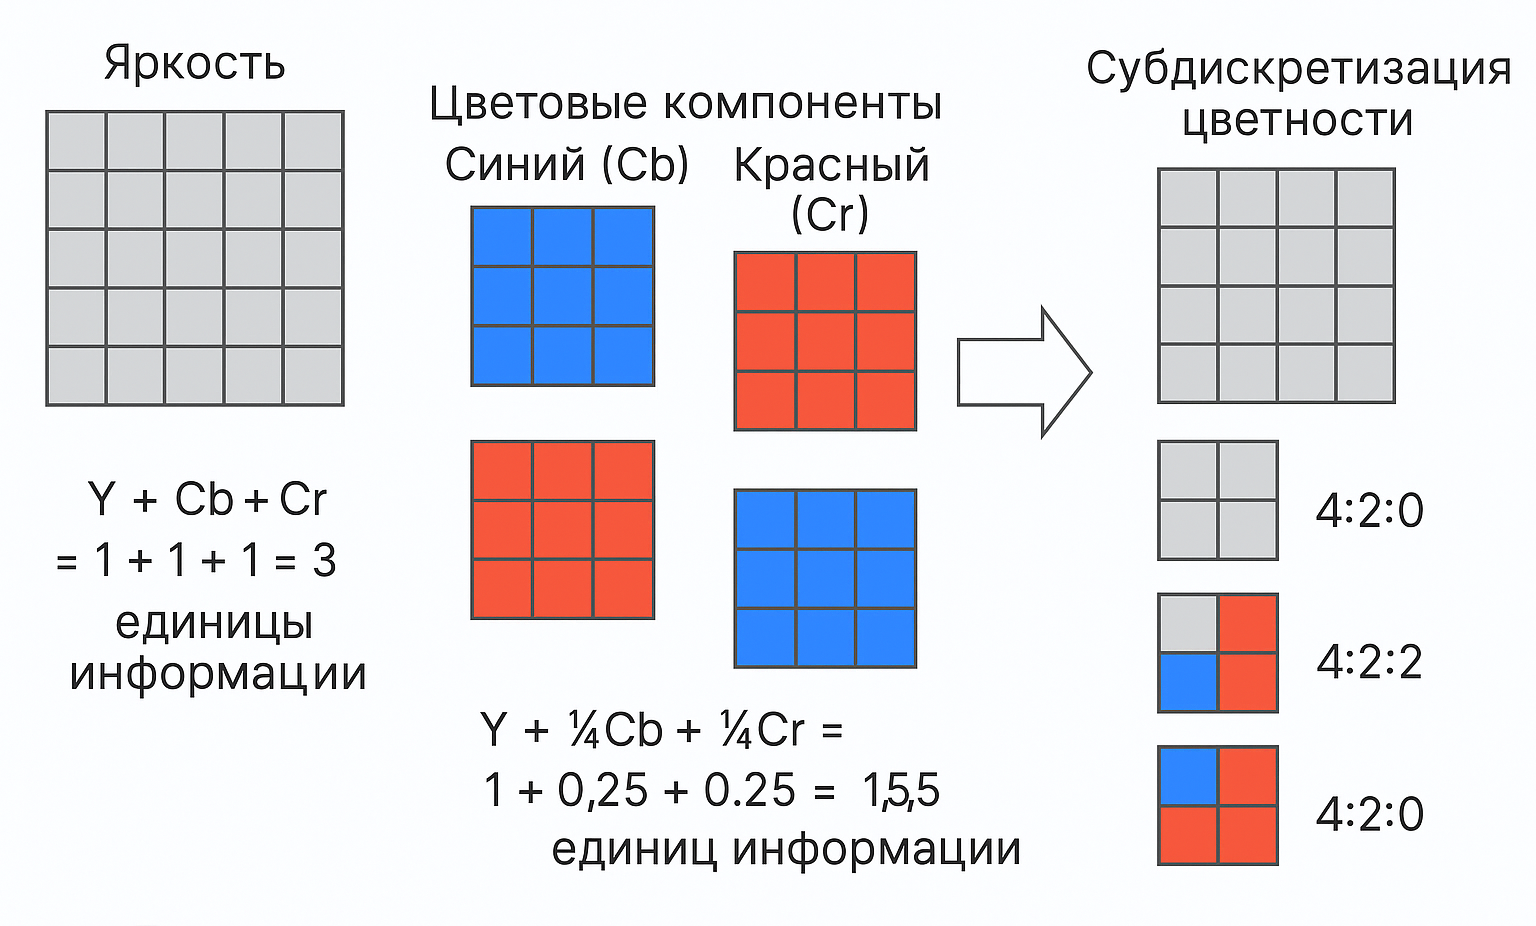
\includegraphics[width=0.7\textwidth]{/home/evgen/Coursework/app/diplom/images/sub_discretization.png}
    \caption{Как происходит преборазование}
    \label{fig:sub_dis}
\end{figure}

Таким образом, достигается двукратное уменьшение общего объёма данных, подлежащих хранению или передаче.

Что важно, такое преобразование происходит практически без визуальных потерь качества. 
Несмотря на то, что цветовые данные редуцируются, человеческий глаз практически не воспринимает различие между оригинальным и сжатым изображением. 
Именно поэтому субдискретизация цветности широко применяется в большинстве алгоритмов сжатия изображений и видео (JPEG, MPEG, H.264),
где критически важно достичь компромисса между качеством и эффективностью хранения данных.

%%%%%%%%%%%%%%%%%%%%%%%%%%%%%%%%%%%%%%%%%%%%%
\subsection{Дискретное косинус-преобразование}

После преобразования изображения из цветового пространства RGB в YCbCr и выполнения хрома-субдискретизации (уменьшения разрешения цветовых компонент Cb и Cr), 
выполняется разбиение изображения на блоки фиксированного размера 8×8 пикселей. 
Однако размеры исходного изображения не всегда кратны восьми, что делает невозможным непосредственное и равномерное разбиение без остатка. 
В таких случаях производится предварительная корректировка размеров изображения: вычисляется необходимое количество дополнительных строк и столбцов, 
которые должны быть добавлены к правому и нижнему краю изображения для достижения кратности 8.

Добавление недостающих строк и столбцов осуществляется с помощью повторения граничных значений (пикселей) изображения, 
чтобы минимизировать искажения, возникающие на краях. 

\AddedBlocks

Этот шаг реализуется при помощи библиотеки OpenCV, предоставляющей функцию для симметричного дополнения изображений. 
После этого скорректированное изображение разбивается на непересекающиеся блоки размером 8×8.

\begin{figure}[H]
    \centering
    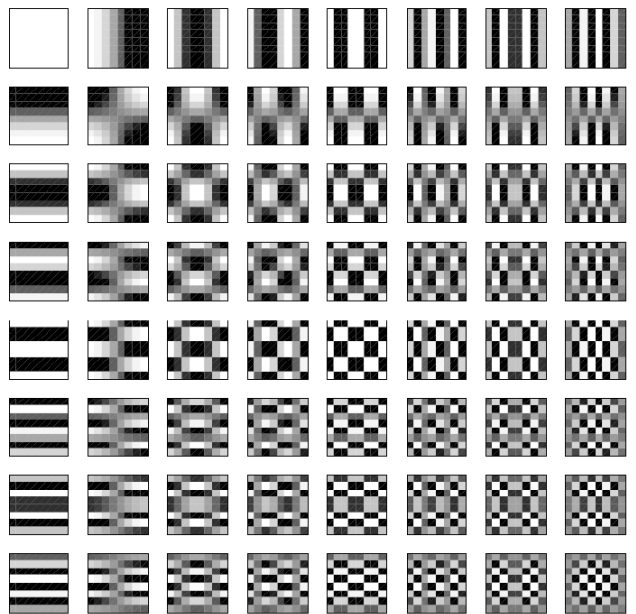
\includegraphics[width=0.7\textwidth]{/home/evgen/Coursework/app/diplom/images/bloks.png}
    \caption{Блоки 8х8}
    \label{fig:blocks}
\end{figure}


Для удобства хранения и последующей обработки эти блоки сохраняются в виде многомерных массивов с использованием библиотеки NumPy. 
Это позволяет эффективно обращаться к отдельным блокам, выполнять над ними математические преобразования и организовать дальнейший процесс.


Это важный шаг, позволяющий значительно повысить эффективность сжатия. 
Разделение на небольшие блоки позволяет применять алгоритмы сжатия локально, что упрощает обработку и улучшает степень компрессии.

Дальнейшая задача заключается в оценке уровня детализации внутри каждого блока. 
Если блок содержит мало визуальных деталей, его можно закодировать с меньшим числом битов, минимизируя потери качества. 
Для анализа степени детализации и выделения значимых компонент используется дискретное косинусное преобразование (ДКП, англ. Discrete Cosine Transform, DCT). 
Преобразование позволяет перейти от пространственного представления блока к частотному, выявляя частотные составляющие, которые имеют наибольшее значение для визуального восприятия.

Для понимания принципов работы ДКП целесообразно сначала рассмотреть его одномерную (векторную) форму, 
поскольку она обладает большей наглядностью и сохраняет все ключевые идеи, лежащие в основе двумерного варианта, применяемого в обработке изображений.


На рисунке~\ref{fig:coswaves}  показано восемь волн косинуса, $\omega(f) = \cos{f \Theta}$, при $0 \leq \Theta \leq \pi$ с частотами $f=0,1,\ldots,7$.

\begin{figure}[h!]
    \centering
    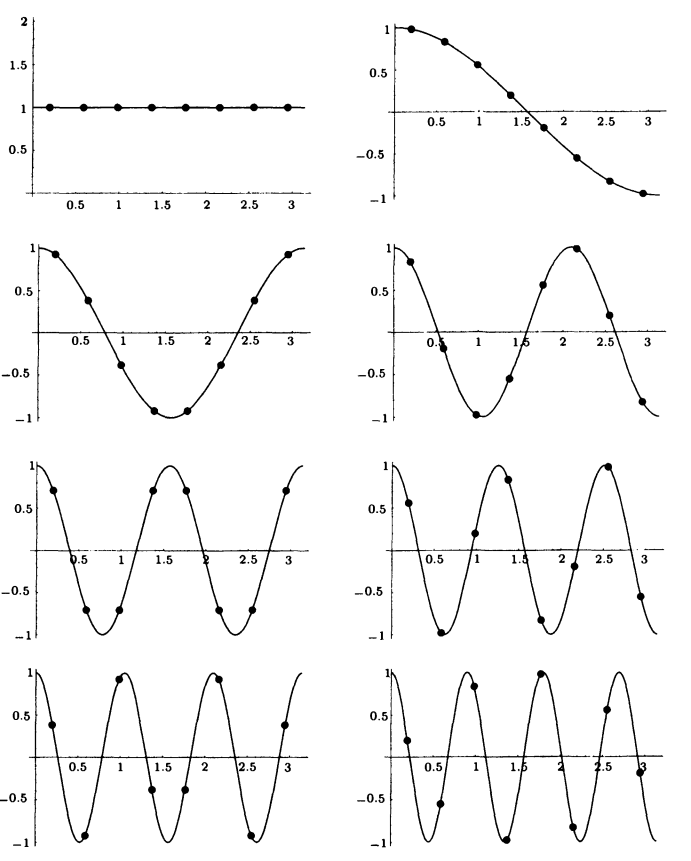
\includegraphics[width=0.7\textwidth]{/home/evgen/Coursework/app/diplom/images/basis_dct.png}
    \caption{Графики функций $\omega(f) = \cos{(f \Theta)}$ для различных частот $f$.}
    \label{fig:coswaves}
\end{figure}

На каждом графике отмечено восемь значений функции $\omega(f)$ с абс­циссами

\begin{equation}
    \Theta = \frac{\pi}{16}, 
                \frac{3\pi}{16}, 
                \frac{5\pi}{16}, 
                \frac{7\pi}{16}, 
                \frac{9\pi}{16}, 
                \frac{11\pi}{16}, 
                \frac{13\pi}{16}, 
                \frac{15\pi}{16}
    \label{eq:theta_values}
\end{equation}


которые формируют базисный вектор $v_f$. В результате получится восемь векторов $v_f, f = 0, 1, \dots, 7$ (всего 64 числа).

\clearpage
\BasisDCT

Они служат базисом одномерного косинусного преобразования, причём частота смены знаков увеличивается по строкам.

Можно показать, что все векторы $v_i$ ортогональны между со­бой (из-за специального выбора восьми точек отсчета $\Theta$). 
То же самое можно обнаружить прямым вычислением с помощью подхо­дящей математической программы. 
Значит, эти восемь векторов можно поместить в матрицу размером 8 на 8 и рассмотреть соот­ветствующее ей ортогональное преобразование - 
вращение в вось­мимерном пространстве, которое называется одномерным дискрет­ным косинус-преобразованием (DCT). 
% Двумерное DCT можно так­же интерпретировать как двойное вращение.////////////////////////////////////////////

Одномерное преобразование косинусов Дискретное (DCT) можно интерпретировать как представление вектора в базисе, состоящем из векторов $v_i$
В этом контексте любой вектор $p$ из соответствующего векторного пространства может быть выражен через линейную комбинацию этих базисных векторов $v_j$.


Например, выберем 8 (коррелированных) чисел $p=(0.6, 0.5, 0.4, 0.5, 0.6, 0.5, 0.4, 0.55)$ в качестве тестовых данных. 
Выразим вектор $p$ в виде суммы $p = \sum_{i}^{} \omega_i v_i$ восьми веторов $v_i$. 
Решив эту систему из 8 линейных уравнений, находим восемь весов

\begin{equation}
    \begin{aligned}
        \omega_0 &=0.506, \omega_1 = 0.0143, \omega_2 = 0.0115, \omega_3 = 0.0439, \\
        \omega_4 &=0.0795, \omega_5 = -0.0432, \omega_6 = 0.00478, \omega_7 = -0.0077.
    \end{aligned}
\end{equation}


Вес $\omega_0$ не сильно отличается от элементов вектора $p$ , но остальные семь весов гораздо меньше. 
Это показывает, как DCT (или любое другое ортогональное преобразование) производит сжатие. 
Теперь можно просто записать эти восемь весов в сжатый файл, 
где онибудут занимать меньше места, чем восемь компонентов исходного вектора $p$.

\begin{figure}[h!]
    \centering
    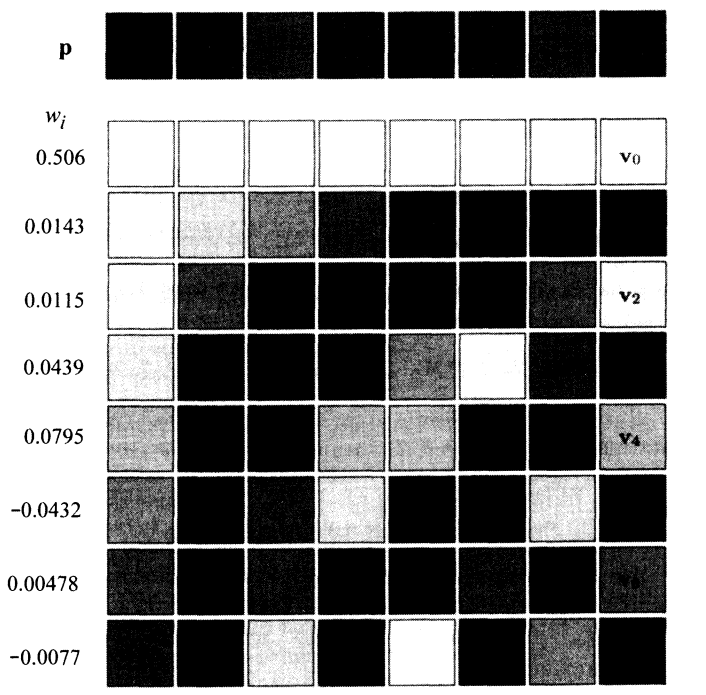
\includegraphics[width=0.7\textwidth]{/home/evgen/Coursework/app/diplom/images/grap_prew_dct.png}
    \caption{Графическое представление одномерного DCT.}
    \label{fig:gr_dt}
\end{figure}

\clearpage
Все восемь векторо $v_i$ показаны в виде ряда из восьми маленьких серых квадратиков,
причем значение $+1$ представлено белым цветом, а значение $-1$ окрашено в ченый цвет. 
Каждый из восьми компонентов вектора $p$ выражен в виде взвешенной суммы восьми серых оттенков.

На практике одномерное DCT проще всего вычислять по формуле

\begin{equation}
    G_f = \frac{1}{2}C_f \sum_{t=0}^{7} p_t \cos{\frac{(2t+1)f \pi}{16}}
    \label{eq:dct}
\end{equation}

$$
\quad \text{где} \quad C_f = 
\left\{
    \begin{array}{ll}
        \frac{1}{\sqrt{2}}, & f = 0, \\
        1, & f > 0. 
    \end{array}
\right.
\quad \text{При} \quad f = 0, 1, \dots, 7.
$$


Здесь исходными данными (пикселами, фрагментами звука или дру­гими элементами) являются величины $p_t$, 
а им соответствующими коэффициентами DCT служат числа $G_f$. 
Формула \eqref{eq:dct} очень про­ста, но процесс вычисления по ней медленный. 
Декодер получает на входе ко­эффициенты DCT, делит их на восьмерки и применяет к ним обрат­ное преобразование DCT (inverse DCT, IDCT) 
для восстановления исходных данных (тоже в виде групп по 8 элементов). Простейшая формула для вычисления IDCT имеет вид

\begin{equation}
    p_t = \frac{1}{2} \sum_{j=0}^{7} C_j G_j \cos{\frac{(2t+1)j \pi}{16}, \text{при} \; t = 0,1, \dots, 7}
\end{equation}


%%%%%%%%%%%%%%%%%%%%%%%%%%%%%%%%%%%%%%%%%%%%%%
\subsection{Двумерное (матричное) DCT}

Из опыта хорошо известно, что пикселы изображения имеют корреляцию  не только по горизонтали, но и по вертикали. 
То есть пиксели взаимосвязаны как с соседними пикселами слева и справа, так и с пикселами сверху и снизу. 
Поэтому методы сжатия изо­бражений используют двумерное DCT, которое задается формулой

\begin{equation}
    G_{ij} = \frac{1}{\sqrt{2n}} C_i C_j\sum_{x=0}^{n-1} \sum_{y=0}^{n-1} p_{xy} \cos{\frac{(2y+1)j \pi}{2n} \cos{\frac{(2x+1)i \pi}{2n}}}
    \label{eq:2D_DCT}
\end{equation}

при $0 \leq i, j \leq n - 1$. Изображение разбивается на блоки пикселов $p_{xy}$ размера $n \times n$ (в данном примере $n = 8$), 
и уравнение \eqref{eq:2D_DCT} используется для нахождения коэффициентов $G_{ij}$ для каждого блока пикселов.
Если частичная потеря информации допустима, то коэффициенты подвергаются квантованию, что будет подробно рассмотрено в следующем разделе. 
Декодер восстанавливает сжатый блок данных (точно или приближенно), вычисляя обратное DCT (IDCT) по формуле


\begin{equation}
    p_{xy} = \frac{1}{4} \sum_{i = 0}^{7} \sum_{j = 0}^{7} C_i C_j G_{ij} \cos{\frac{(2y+1)j \pi}{16} \cos{\frac{(2x+1)i \pi}{16}}}
    \label{eq:I2D_DCT}
\end{equation}

$$
\quad \text{где} \quad C_f = 
\left\{
    \begin{array}{ll}
        \frac{1}{\sqrt{2}}, & f = 0, \\
        1, & f > 0. 
    \end{array}
\right.
$$


Двумерное дискретное косинусное преобразование (DCT) можно интерпретировать двумя способами: как композицию двух вращений, 
а также через представление вектора в базисе $n$-мерного векторного пространства. 
В первой ин­терпретации используется блок $n \times n$ пикселов (рис. \eqref{fig:coefs}a, где элементы обозначены буквой "L")


\begin{figure}[h!]
    \centering
    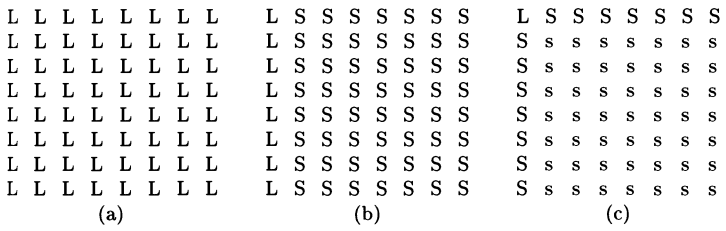
\includegraphics[width=0.7\textwidth]{/home/evgen/Coursework/app/diplom/images/coef_blocks.png}
    \caption{Двумерное DCT и двойное вращение.}
    \label{fig:coefs}
\end{figure}


Сначала рассматриваются строки этого блока как точки $(p_{x,0}, p_{x,1}, \dots, p_{x,n-1})$ в $n$- мерном пространстве,
которые поворачиваются в этом пространстве с помощью преобразования, задаваемого внутренней суммой

$$
G1_{x,j} = C_j \sum_{y=0}^{n-1} p_{xy} \cos{\frac{(2y+1)j \pi}{2n}}
$$


из уравнения \eqref{eq:2D_DCT}. Результатом этого вращения служит блок $G1_{x,j}$ из $n \times n$ коэффициентов, 
в котором в строках доминируют первые элементы (обозначенные как «L» на рис. \eqref{fig:coefs}b), 
в то время как все остальные элементы малы (они обозначены как «S»). Внешняя сумма, приведенная в уравнении \eqref{eq:2D_DCT}, равна


$$
G_{ij} = \frac{1}{\sqrt{2n}} C_i \sum_{x=0}^{n-1} p_{xy} G1_{x,j} \cos{\frac{(2x+1)i \pi}{2n}}
$$

Здесь уже столбцы матрицы $1_{x,j}$ рассматриваются в качестве то­чек $n$ - мерного векторного пространства, над которыми совершает­ся преобразование вращения. 
В результате получается один боль­шой коэффициент в верхнем левом углу блока (на рис.\eqref{fig:coefs}c - это «L») 
и $N^2 - 1$ маленьких коэффициентов в остальных местах («S» и «s» на рисунке). 
Эта интерпретация рассматривает двумерное DTC в виде двух разных вращений размерности $n$. 


Вторая интерпретация (при $n = 8$) использует уравнение \eqref{eq:2D_DCT} для создания 64 блоков по $8 \times 8$ величин в каждом. 
Все 64 блока рас­сматриваются в качестве базиса 64-мерного векторного простран­ства (это базисные изображения). 
Любой блок $B$ из $8 \times 8$ пикселов можно выразить как линейную комбинацию этих базисных изобра­жений, 
и все 64 веса этой линейной комбинации образуют коэффи­циенты DCT блока $B$.


\begin{figure}[h!]
    \centering
    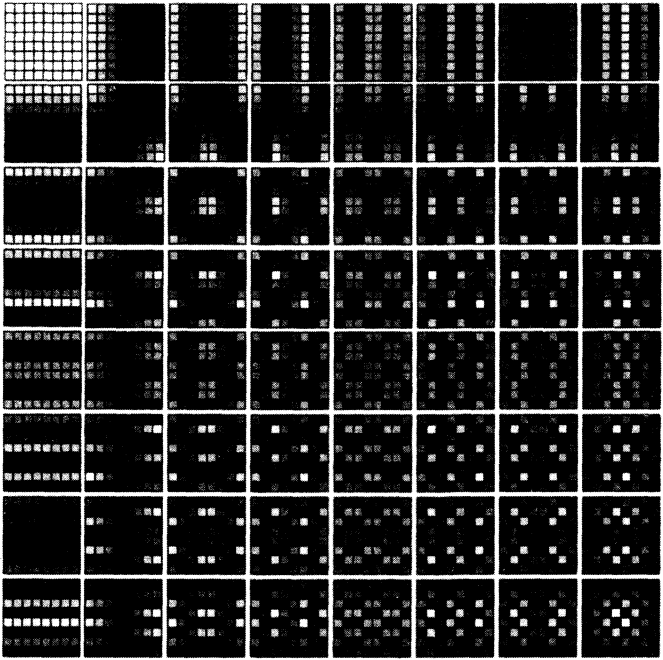
\includegraphics[width=0.7\textwidth]{/home/evgen/Coursework/app/diplom/images/basis2dDCT.png}
    \caption{64 базисных изображения двумерного DCT.}
    \label{fig:basis2dDCT}
\end{figure}


На рисунке выше представлено графическое отображение 64 базисных функций 
двумерного дискретного косинусного преобразования (DCT) при размере блока $n=8$.
 Каждый элемент с координатами $(i,j)$ на данном рисунке соответствует блоку размером $8 \times 8$, 
 полученному в результате вычисления выражения $\cos{(i \cdot s)} \cdot \cos{(j \cdot t)}$, 
 где переменные $s$ и $t$ изменяются независимо в пределах, определённых уравнением \eqref{eq:theta_values}.\\


 Подведем итог этого, довольно сложного шага. Сжатие любого изображения с помощью DCT можно теперь сделать следующим образом.


 \begin{enumerate}
    \item Разделить изображение на $k$ блоков пикселов размером $n \times n$ (чаще всего используется размер $8 \times 8)$.
    \item Применить дискретное косинусное преобразование (DCT) к каждому блоку $B^{(i)}$, представив его в виде линейной комбинации
    64 базисных функций, показанных на рисунке выше. В результате получится набор блоков (далее будем называть их векторами) $W^{(i)}$,
    каждый из которых содержит 64 коэффициента $\omega^{(i)}_{j}$, где $j = 0, 1, \dots, 63$.
    \item Векторы $W^{(i)}$, где $i = 1, 2, \dots, k$, группируются по компонентам, формируя 64 отдельных вектора коэффициентов
    $$
    \mathbf{C_j} = \{ \omega^{(1)}_j, \omega^{(2)}_j, \dots, \omega^{(k)}_j \}.
    $$
    В частности, вектор $\mathbf{C_0}$ состоит из $k$ коэффициентов DC.
    \item Каждый вектор коэффициентов $C^{(j)}$ подвергается квантованию независимо от остальных. 
    Полученные квантованные векторы $Q^{(j)}$ далее могут быть дополнительно сжаты с использованием методов, 
    таких как RLE, код Хаффмана или других алгоритмов, и записаны в сжатый файл.
 \end{enumerate}



%%%%%%%%%%%%%%%%%%%%%%%%%%%%%%%%%%%%%%%%%%%%%%
\subsection{Квантование}

В процессе сжатия изображений важным этапом является \textbf{квантование}, 
под которым понимается преобразование чисел с высокой точностью (чаще всего вещественных) в значения с меньшей точностью, 
например — округление до ближайшего целого или замена на приближённое значение из ограниченного набора. 

Это позволяет существенно уменьшить объём передаваемой или сохраняемой информации за счёт исключения наименее значимых деталей, 
воспринимаемых человеком слабо либо вовсе незаметных.

Существует два основных подхода к квантованию — \textbf{скалярное} и \textbf{векторное}.

\textbf{Скалярное} квантование представляет собой поэлементную обработку данных, 
когда каждое значение преобразуется независимо от других. 
Этот метод прост в реализации и интуитивно понятен, но не всегда обеспечивает оптимальный результат: 
полезная информация может быть утеряна даже в значимых фрагментах, если не учитывать взаимосвязь между соседними значениями.

Для повышения эффективности используется \textbf{векторное} квантование, где обрабатываются не отдельные числа, 
а целые блоки данных — группы пикселей, которые рассматриваются как многомерные векторы. 
Перед началом сжатия формируется специальный набор типовых блоков — кодовая книга. 
Каждый блок изображения сравнивается со всеми элементами этой книги, и выбирается наиболее близкий (в смысле минимальной разности значений). 
Вместо самого блока в выходной поток данных записывается лишь индекс (или указатель) соответствующего эталонного блока из кодовой книги.

Поскольку индекс, как правило, занимает меньше места, чем полный блок, такой подход позволяет добиться существенного уменьшения размера изображения. 
При этом достигается разумный баланс между степенью сжатия и качеством восстановления, 
особенно если кодовая книга заранее адаптирована под характеристики изображений, с которыми предполагается работать.

В стандарте JPEG реализовано канально-зависимое скалярное квантование, при котором каждый коэффициент, 
полученный в результате дискретного косинусного преобразования (DCT), квантуется независимо от остальных. 
Для каждого из цветовых компонентов — яркостного ($Y$) и двух хроминансных ($Cb$ и $Cr$) — применяются отдельные квантовочные матрицы, 
отражающие различную чувствительность человеческого зрения к яркости и цвету. 
Эти матрицы сформированы на основе психовизуальных моделей и оптимизированы так, 
чтобы минимизировать визуально заметные искажения при сжатии.

\YQuantize

\CbCrQuantize

Избыточное квантование может привести к появлению блочных артефактов, особенно при низком битрейте. 
Эти артефакты возникают из-за чрезмерной потери информации в результатах квантования и часто становятся заметными на границах блоков.

Когда коэффициенты в матрице квантования слишком велики (например, при слишком сильном сжатии), 
значительная часть информации теряется, особенно в высокочастотных компонентах, которые отвечают за детали изображения. 
Этот процесс квантования приводит к значительным потерям точности в преобразованных данных. 
На изображении это выражается в виде артефактов, которые часто становятся видимыми в местах стыка блоков.

Однако, такого эффекта можно добитья и при слишком малом квантовании.
На границах блоков, где алгоритм не может точно передать информацию, 
начинается видимый переход между различными уровнями яркости или цвета, 
что приводит к образованию четких линий или квадратных паттернов, которые визуально ощущаются как артефакты.

Так же, поскольку изображение разбивается на блоки размером $8 \times 8$ пикселей, и каждый блок сжимается независимо. 
Это может привести к потере контекста между блоками, особенно в случае сильного сжатия. 
Границы блоков не могут быть плавными, из-за чего возникают резкие переходы между блоками.

Эти артефакты могут выглядеть как "ступеньки" или резкие изменения яркости и цвета, которые не присутствуют в исходном изображении.

\subsubsection{Как уменьшить блочные артефакты}

Существует несколько подходов для минимизации блочных артефактов при сжатии JPEG:
\begin{enumerate}
    \item Использование более низкого коэффициента сжатия: Уменьшение уровня сжатия помогает сохранить больше данных, 
    что уменьшает квантование и, соответственно, количество потерь информации. 
    Это снижает вероятность появления артефактов, но увеличивает размер файла.

    \item Адаптивное квантование: В некоторых случаях используется адаптивное квантование, 
    при котором для разных частей изображения выбираются различные матрицы квантования в зависимости от содержания. 
    Например, для областей с высокой детализацией можно использовать более точное квантование, а для равномерных областей — более грубое.

    \item Эксперименты с постобработкой: В некоторых случаях для устранения артефактов применяются методы постобработки, такие как сглаживание или фильтрация на уровне блоков.

    \item Использование более сложных алгоритмов сжатия: Алгоритмы сжатия, такие как JPEG2000, 
    используют более сложные методы, которые могут уменьшить или полностью устранить блочные артефакты. 
    В частности, JPEG2000 использует вейвлет-преобразования вместо DCT, что позволяет избежать проблемы разделения изображения на блоки и улучшить качество сжатия.
\end{enumerate}

\vspace{1em}

JPEG не использует векторное квантование в силу его значительно большей вычислительной и алгоритмической сложности: 
построение и оптимизация кодовой книги требуют значительных ресурсов, 
а сам процесс кодирования с подбором ближайшего эталона становится существенно менее эффективным для реализации в массовых форматах хранения изображений. 
Кроме того, векторное квантование хуже адаптируется к переменной структуре изображений и менее совместимо с блочной природой DCT-представления.




%%%%%%%%%%%%%%%%%%%%%%%%%%%%%%%%%
\subsection{Зигзаг-преобразование блоков}

После применения DCT, и последующего квантования блоков, изображение представляется в виде матрицы коэффициентов $8 \times 8$, 
где каждый коэффициент представляет собой степень различной частоты. 
Эти коэффициенты могут включать как высокочастотные (мелкие детали изображения), так и низкочастотные компоненты (общие очертания). 
Важным моментом является то, что после квантования высокочастотные коэффициенты, как правило, имеют значения, близкие к нулю, 
и не играют значительной роли для восприятия изображения. 
Поэтому их можно исключить или закодировать с меньшей точностью.

Зигзаг-преобразование используется для того, чтобы упорядочить эти коэффициенты в порядке, 
который позволяет более эффективно их кодировать. 
Суть метода в том, что он позволяет собирать все нулевые значения (или значения, близкие к нулю) в конец последовательности, 
что снижает объем данных при их дальнейшем кодировании.

Зигзаг-преобразование упорядочивает эти коэффициенты таким образом, что сначала идут наиболее значимые коэффициенты (низкочастотные), 
а затем — менее значимые (высокочастотные, которые в основном равны нулю).

Зигзагообразный порядок включает следующие шаги:

\begin{enumerate}
    \item Начинается с первого элемента в верхнем левом углу матрицы (нулевой индекс).
    \item Затем происходит движение по диагоналям матрицы, начиная с верхней левой части, последовательно переходя к правому нижнему углу.
    \item Каждая диагональ матрицы представляет собой группу коэффициентов, которые последовательно вытягиваются в одном ряду.
\end{enumerate}


\begin{figure}[h!]
    \centering
    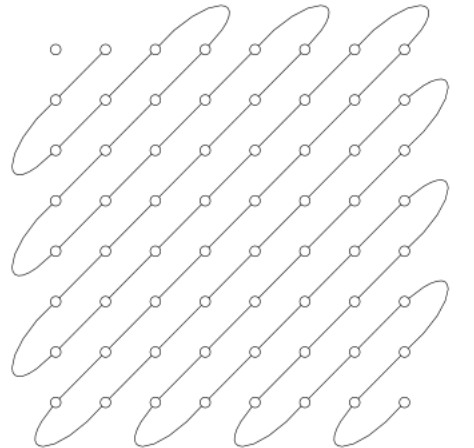
\includegraphics[width=0.7\textwidth]{/home/evgen/Coursework/app/diplom/images/zig_zag.png}
    \caption{Обход блока зиг-заг.}
    \label{fig:zig_zag}
\end{figure}


В результате применения зигзагообразного обхода к блоку преобразованных коэффициентов 
дискретного косинусного преобразования формируется линейная последовательность. Один из примеров такой последовательности приведён ниже.

\begin{equation}
    \label{eq:zigzag_example}
    \text{Последовательность после зигзагообразного обхода: } 
    \left\{
    \begin{array}{cccccccc}
    52 & -3 & 0 & 0 & 0 & 2 & 0 & 0 \\
    0 & 0 & 0 & 0 & 0 & 0 & 1 & 0
    \end{array}
    \right\}
    \end{equation}

Здесь первый элемент (52) соответствует DC-компоненте, а последующие значения — коэффициенты высоких частот (AC-компоненты), 
отсортированные по убыванию их вклада в общее изображение.


%%%%%%%%%%%%%%%%%%%%%%%%%%%%%%%%%
\subsection{RLE-кодирование}


После применения зигзаг-преобразования каждый блок коэффициентов преобразуется в одномерный массив, 
в котором значимая информация (низкочастотные коэффициенты) сосредоточена в начале, 
а большая часть оставшихся элементов принимает нулевое значение. 
Это делает полученную последовательность особенно удобной для дальнейшего сжатия с использованием методов, 
предназначенных для работы с повторяющимися элементами.

На этом этапе в классическом алгоритме JPEG традиционно применяется энтропийное кодирование, 
наиболее часто — с использованием кода Хаффмана, 
позволяющего достичь высокой степени сжатия за счёт построения оптимального префиксного кодового дерева, 
основанного на вероятностях появления различных значений. 
Однако реализация эффективного кодировщика Хаффмана требует значительных трудозатрат, 
включая построение статистической модели, генерацию кодовых деревьев и реализацию соответствующего декодирования.

В рамках данной работы энтропийное кодирование было намеренно опущено. 
Вместо него используется более простой и наглядный метод кодирования с повторениями — Run-Length Encoding (RLE), 
который позволяет проиллюстрировать фундаментальные принципы постобработки данных после зигзаг-преобразования и обеспечивает компрессию, 
достаточную для демонстрации эффективности базового JPEG-подобного сжатия. 
Это решение продиктовано необходимостью сосредоточиться на ключевых этапах сжатия и ограниченностью временных ресурсов, 
отведённых на реализацию дипломного проекта.

Применение RLE особенно эффективно в контексте JPEG-подобного представления данных, 
так как вследствие квантования и зигзагообразного упорядочивания большинство коэффициентов в конце последовательности равны нулю.
Алгоритм RLE преобразует такие повторы в компактную форму, 
заменяя длинные последовательности одинаковых значений (в первую очередь нулей) парой «значение–длина повтора», 
что существенно снижает объём итоговых данных.

Таким образом, хотя в полномасштабной реализации алгоритма JPEG предпочтительно использовать энтропийное кодирование, 
в рамках данной работы RLE выступает как более простая альтернатива, 
позволяющая сохранить общий принцип компрессии без существенного увеличения сложности реализации.


\begin{RLETable}
\end{RLETable}


\begin{RLEEncodedTable}
\end{RLEEncodedTable}


Применение RLE позволяет существенно сократить объём информации, подлежащей сохранению или передаче, 
при этом сохраняя возможность точного восстановления исходной последовательности. 
Хотя степень сжатия, достигаемая с помощью RLE, уступает алгоритмам энтропийного кодирования (таким как Хаффман), 
его простота и наглядность делают его отличным выбором для учебных и демонстрационных целей.

Таким образом, использование RLE в данной работе позволило реализовать полный цикл JPEG-подобного сжатия — от разделения изображения 
на блоки и применения косинус-преобразования до финального этапа кодирования, — при этом сосредоточившись на ключевых принципах без 
чрезмерного усложнения алгоритма.



%%%%%%%%%%%%%%%%%%%%%%%%%%%%%%%%%%%%%%%%%%%%%%%%%%%
\subsection{Декодирование}

Процесс декодирования JPEG является обратной операцией по отношению к этапам кодирования
и направлен на восстановление изображения из сжатого представления. 
На выходе должен быть получен массив пикселей, максимально приближенный к исходному изображению. 
Процесс декодирования включает следующие этапы:

 
\subsubsection{Распаковка закодированных данных}

На первом этапе декодирования выполняется извлечение и интерпретация сжатых данных, 
полученных после применения метода RLE (run-length encoding, кодирование длин серий). 
В процессе кодирования многие коэффициенты DCT, особенно высокочастотные, равны нулю. 
Это свойство используется для повышения степени сжатия — нули заменяются на пары вида (количество нулей, ненулевое значение).

При декодировании производится восстановление полного набора коэффициентов блока размером $8 \times 8$
из такой сжатой последовательности. Например, последовательность:

\begin{equation}
    \label{eq:rle_example}
    \begin{aligned}
        &\text{Сжатая последовательность пар (количество нулей, значение):} \\
        &\qquad (0,\ 52),\ (0,\ -3),\ (3,\ 2),\ (9,\ 1) \\
        &\text{После распаковки:} \\
        &\qquad 52,\ -3,\ 0,\ 0,\ 0,\ 2,\ 0,\ 0,\ 0,\ 0,\ 0,\ 0,\ 0,\ 0,\ 1,\ 0
    \end{aligned}
\end{equation}



\subsubsection{Обратный зигзагообразный обход}
Поскольку в процессе кодирования двумерный массив коэффициентов представлялся в виде одномерного массива 
с помощью зигзагообразного обхода, теперь необходимо восстановить исходное расположение коэффициентов в блоке $8 \times 8$. 
Каждому элементу последовательности возвращается его позиция в соответствии со стандартной зигзагообразной схемой.




\subsubsection{Обратное квантование}
На этапе обратного квантования каждый коэффициент умножается на соответствующее значение из таблицы квантования, 
использованной при кодировании. Если обозначить квантованный коэффициент как $Q_{i,j}$, а таблицу квантования как $T_{i,j}$,
то восстановленный DCT-коэффициент можно получить по формуле:

\begin{equation}
    D_{i,j} = Q_{i,j} \cdot T_{i,j}
\end{equation}

Это приближает коэффициенты к их исходным значениям до потери точности при квантовании.




\subsubsection{Обратное дискретное косинусное преобразование (IDCT)}
На этом этапе выполняется обратное дискретное косинусное преобразование (IDCT) для каждого блока. 
Восстановление значений пикселей в пространственной области осуществляется на основе 64 DCT-коэффициентов, по формуле \eqref{eq:I2D_DCT}.


\subsubsection{Восстановление блоков}
После применения IDCT к каждому блоку получаются блоки из 64 значений интенсивности, которые собираются в итоговое изображение. 
При этом важно точно соблюсти позиционирование блоков и границы изображения.

После этого идет обратное преобразование цветного пространства из $\textbf{YCbCr}$ в $\textbf{RGB}$, 
что позволяет получить восстановленное изображение в привычном для восприятия формате.

% Однако, несмотря на сложность и точность процесса декодирования, JPEG не всегда идеален для всех типов изображений. 
% Алгоритм сжатия может проявлять свои ограничения, 
% особенно в случае с изображениями с ярко выраженными границами и резкими переходами, где заметны артефакты, 
% такие как блоковые искажения. 
% Эти ограничения обусловлены особенностями самого алгоритма, 
% который оптимизирован для сжатия изображений с плавными переходами и небольшими деталями, 
% но может не справляться с сохранением чёткости на изображениях с высококонтрастными зонами.

% Таким образом, несмотря на высокую эффективность JPEG и его широкое распространение, 
% в специфических случаях, таких как изображения с четкими линиями и границами, алгоритм может показывать свои слабые стороны. 
% В таких ситуациях целесообразно использование вариации параметров на разных этапах алгоритма.
% Можно пробовать изменять коэффициент сжатия на этапе квантования или менять размер блока при разбиении.
% В некоторых случаях используется адаптивное квантование, 
% при котором для разных частей изображения выбираются разные матрицы квантования в зависимости от содержания.
% Для устранения артефактов после сжатия применяются методы постобработки, такие как сглаживание или фильтрация на уровне блоков, 
% что помогает улучшить визуальное восприятие изображения.

% Помимо этого, существуют более продвинутые алгоритмы сжатия, которые изначально ориентированы на устранение подобных недостатков. 
% Так, например, JPEG2000 использует вейвлет-преобразования вместо DCT, 
% что позволяет избежать деления изображения на независимые блоки. 
% Это снижает вероятность появления блоковых артефактов и обеспечивает более высокое качество сжатия при сопоставимом уровне потерь.

% --- Программная реализация, руководство пользователя
\section{Руководство пользователя}

\subsection{Назначение программы}

Разработанная программа реализует алгоритм сжатия изображений, повторяющий основные этапы стандарта JPEG. 
В отличие от оригинального алгоритма, на этапе энтропийного кодирования используется метод RLE (Run-Length Encoding) 
вместо кодирования по Хаффману. 
Это позволяет упростить реализацию, сохранив при этом все основные свойства алгоритма JPEG.

Программа предназначена для демонстрации полного цикла кодирования и декодирования изображения:

\begin{itemize}
    \item переход от $\textbf{RGB}$ к $\textbf{YCbCr}$
    \item разбиение на блоки $8 \times 8$
    \item дискретное косинус-преобразование (DCT)
    \item квантование
    \item последовательное сканирование (зигзаг)
    \item кодирование RLE
    \item обратные преобразования (IDCT и т. д.)
    \item восстановление RGB-изображения

\end{itemize}



\clearpage
%%%%%%%%%%%%%%%%%%%%%%%%%%%%%%%%%%%%%%%%%%%%%%%%
\subsection{Интерфейс программы}

На рисунке ~\ref{fig:interface} представлено главное окно приложения.

\begin{figure}[h!]
    \centering
    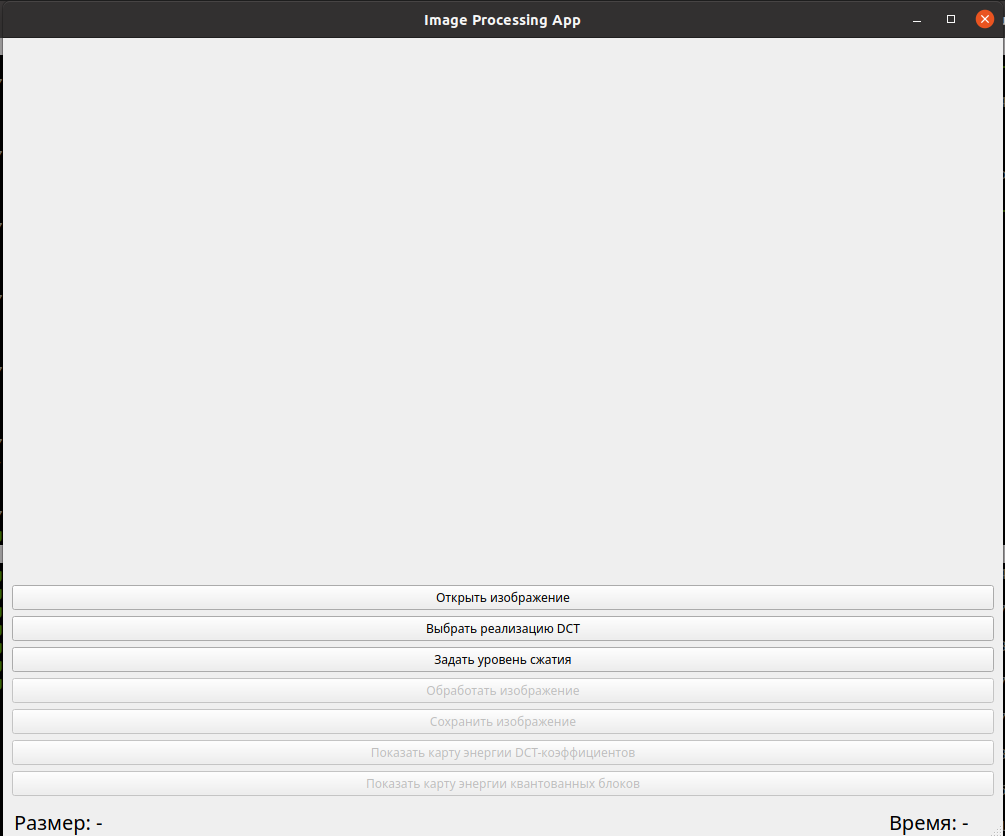
\includegraphics[width=0.7\textwidth]{/home/evgen/Coursework/app/diplom/images/interface.png}
    \caption{Главное окно приложения.}
    \label{fig:interface}
\end{figure}



\subsubsection{Основные элементы интерфейса:}

\begin{itemize}
    \item \textbf{Открыть изображение}

    Позволяет выбрать изображение в формате PNG или JPEG для обработки.
    
    \begin{figure}[h!]
        \centering
        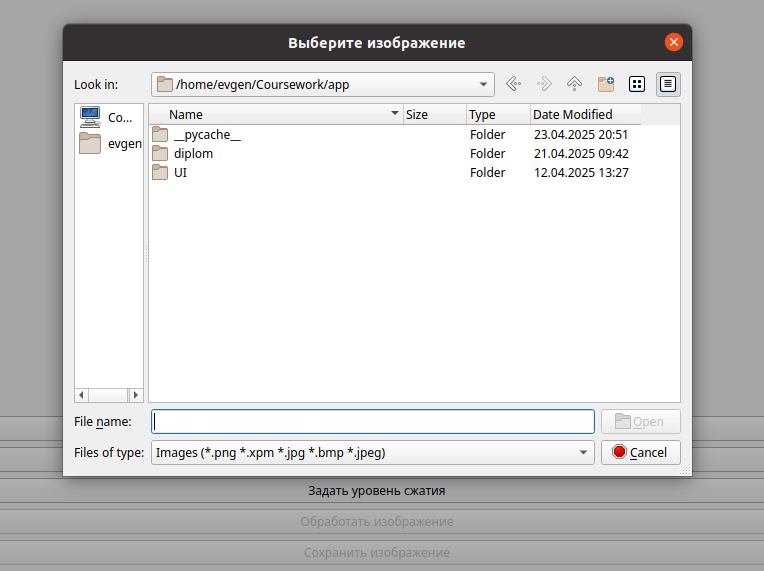
\includegraphics[width=0.5\textwidth]{/home/evgen/Coursework/app/diplom/images/win_choice.png}
        \caption{Окно выбора изображений.}
        \label{fig:win_choice}
    \end{figure}



    \item \textbf{Выбрать реализацию DCT}

    В графическом интерфейсе приложения предусмотрена возможность выбора реализации дискретного косинусного преобразования (DCT). 
    Пользователю предлагаются два варианта:

    Собственная реализация DCT, разработанная вручную в рамках дипломного проекта;
    
    Готовая реализация из библиотеки SciPy (scipy.fftpack.dct), используемая в качестве эталонной и производительной альтернативы.
    
    Это позволяет провести наглядное сравнение корректности и эффективности обеих реализаций, а также удостовериться в соответствии собственной реализации общепринятым стандартам.

    \begin{figure}[h!]
        \centering
        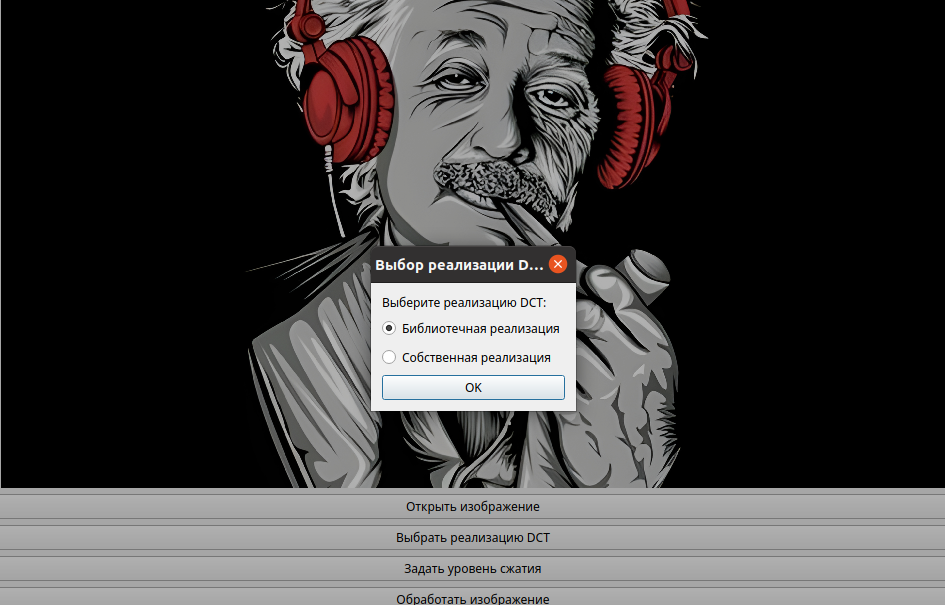
\includegraphics[width=0.8\textwidth]{/home/evgen/Coursework/app/diplom/images/choice_dct.png}
        \caption{Выбрать реализацию DCT.}
        \label{fig:choice_dct}
    \end{figure}



    \item \textbf{Задать уровень сжатия}
    
    Предусмотрена возможность установки уровня сжатия, который напрямую влияет на коэффициенты квантования. 
    Более высокий уровень сжатия приводит к агрессивному округлению высокочастотных коэффициентов, 
    что уменьшает объём выходного файла, но может снизить качество восстановленного изображения. 
    Напротив, меньшие значения сохраняют больше информации, обеспечивая лучшее качество при увеличенном размере файла.

    Это позволяет пользователю находить баланс между качеством изображения и степенью компрессии в зависимости от задач.
    \begin{figure}[h!]
        \centering
        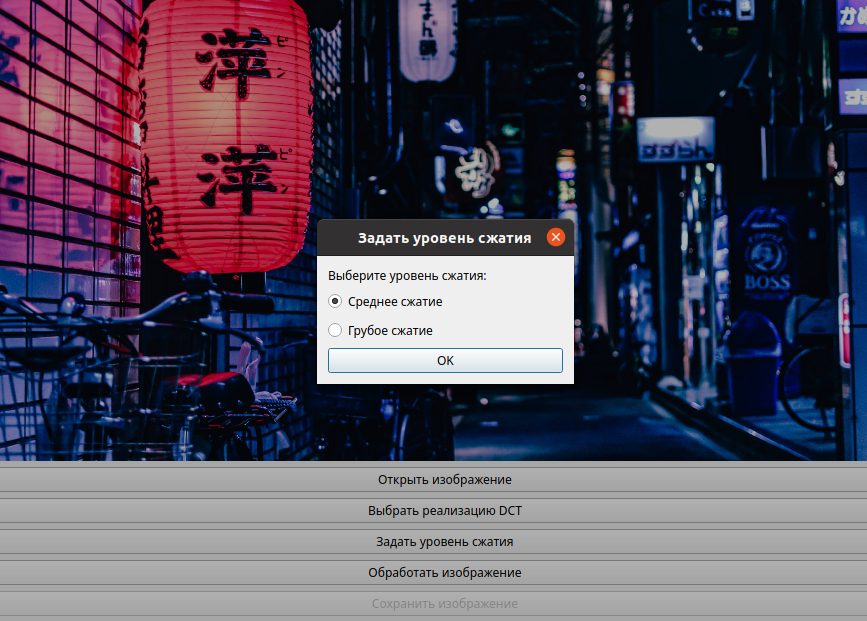
\includegraphics[width=0.9\textwidth]{/home/evgen/Coursework/app/diplom/images/lvl_compres.png}
        \caption{Выбрать уровень сжатия.}
        \label{fig:lvl_compres}
    \end{figure}

    \FloatBarrier

    \item \textbf{Обработать изображение}
    
    После выбора параметров пользователь может запустить процесс обработки, 
    нажав на кнопку \textbf{«Обработать изображение»}. 
    Программа выполняет полный цикл сжатия и восстановления изображения, повторяя основные этапы алгоритма JPEG.

    Сначала изображение преобразуется из цветового пространства RGB в YCbCr.
    Затем изображение разбивается на блоки.
    К каждому блоку применяется дискретное косинусное преобразование (DCT), 
    переводя данные из пространственной области в частотную. 
    Полученные коэффициенты проходят этап квантования, 
    при котором незначительные высокочастотные компоненты подавляются — это и есть основное сжатие с потерями.

    После квантования коэффициенты сканируются по зигзагообразной траектории, что группирует нули, 
    появившиеся в результате округлений. 
    Затем выполняется кодирование методом RLE.

    На финальном этапе происходит декодирование, и вывод получившегося изображения в в окне приложения.

    \begin{figure}[h!]
        \centering
        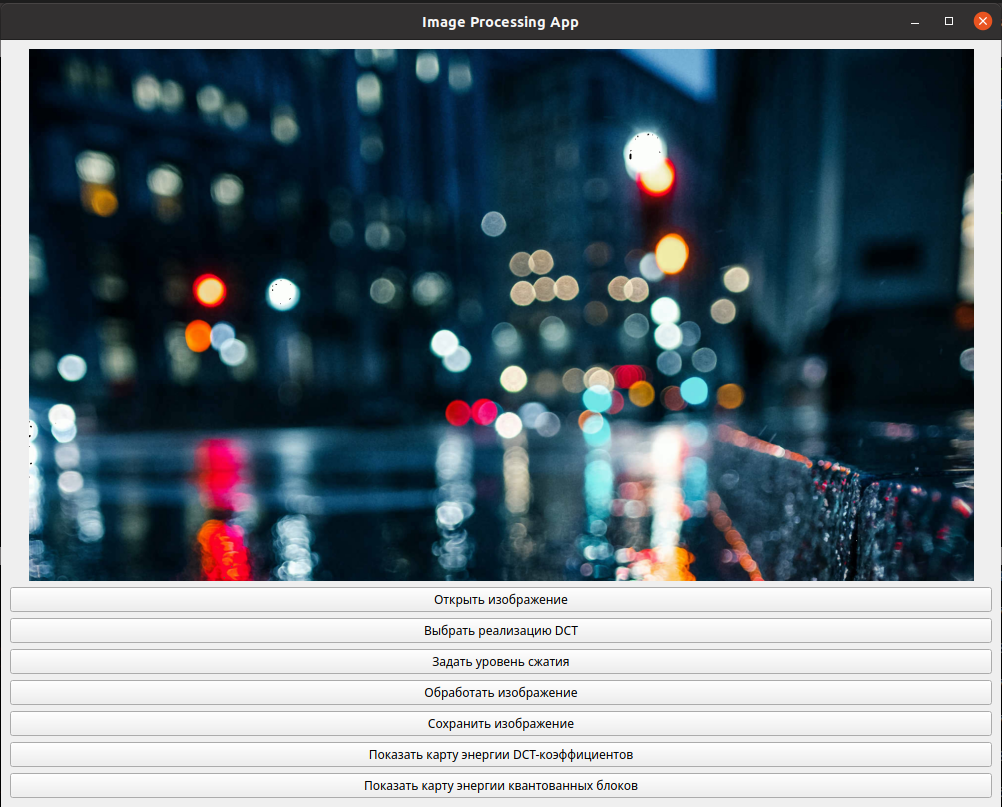
\includegraphics[width=0.9\textwidth]{/home/evgen/Coursework/app/diplom/images/continue.png}
        \caption{Дополнительные элементы.}
        \label{fig:continue}
    \end{figure}


    После завершения обработки становятся доступными дополнительные элементы интерфейса, 
    позволяющие более подробно проанализировать результат.

    \FloatBarrier

    \item \textbf{Сохранить изображение}
    
    Позволяет сохранить на диске восстановленное после сжатия изображение в формате JPEG.

    \begin{figure}[h!]
        \centering
        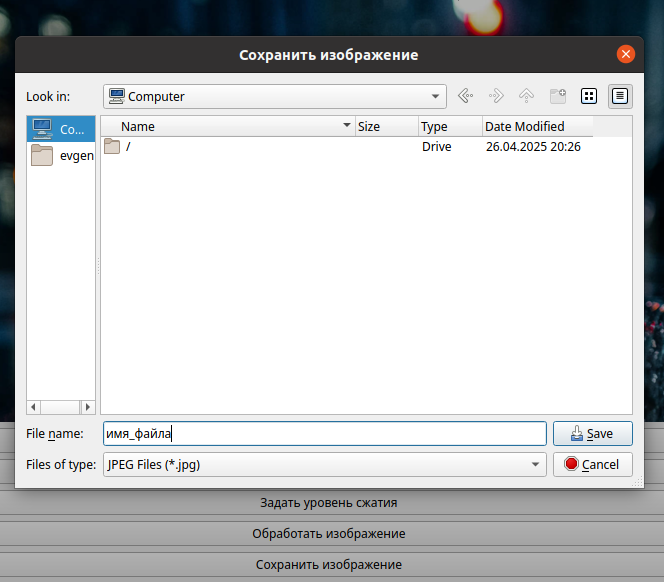
\includegraphics[width=0.9\textwidth]{/home/evgen/Coursework/app/diplom/images/save_img.png}
        \caption{Сохранить изображение.}
        \label{fig:save_img}
    \end{figure}


    \FloatBarrier
    \item \textbf{Показать карту энергии DCT-коэффициентов}
    
    Данный элемент визуализирует вклад различных частотных компонент в изображение до этапа квантования. 
    Это позволяет понять, какие частоты наиболее значимы в передаче визуальной информации


    \begin{figure}[h!]
        \centering
        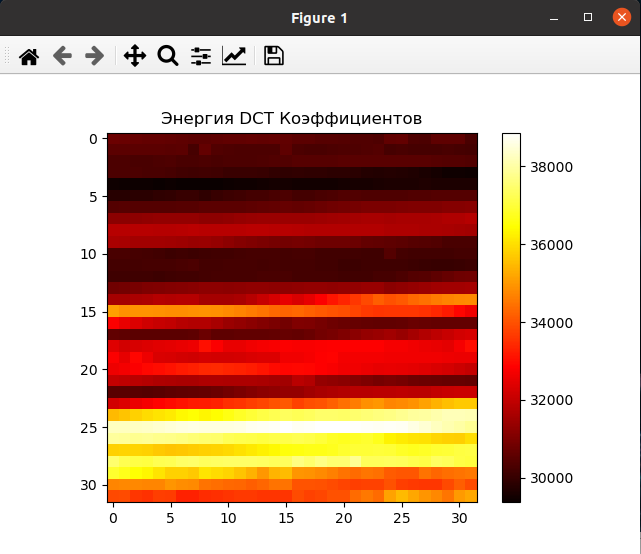
\includegraphics[width=0.9\textwidth]{/home/evgen/Coursework/app/diplom/images/map_energy.png}
        \caption{Карта энергии DCT-коэффициентов.}
        \label{fig:map_energy}
    \end{figure}


    \FloatBarrier

    \item \textbf{Показать карту энергии квантованных блоков} 

    Отображает распределение энергии после квантования. 
    Данная визуализация помогает оценить потери, вызванные округлением коэффициентов.

    \begin{figure}[h!]
        \centering
        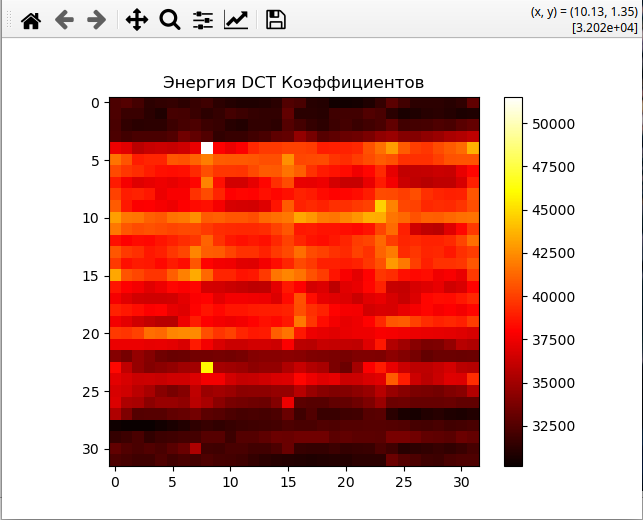
\includegraphics[width=0.9\textwidth]{/home/evgen/Coursework/app/diplom/images/map_quant.png}
        \caption{Карта энергии квантованных блоков.}
        \label{fig:map_quant}
    \end{figure}

\end{itemize}

\FloatBarrier
В нижней части окна приложения отображаются числовые параметры, 
предоставляющие пользователю информацию о производительности и эффективности алгоритма сжатия:
\begin{itemize}
    \item \textbf{Размер изображений} — отображает объём изображения до и после обработки, в килобайтах. 
    Этот позволяет пользователю сравнить исходный размер файла с результатом сжатия и оценить, 
    насколько сильно уменьшился объём данных.

    \item \textbf{Время обработки} — показывает общее время, затраченное на выполнение всех этапов алгоритма, 
    включая преобразование цветового пространства, разбиение на блоки, дискретное косинусное преобразование, 
    квантование, кодирование с помощью RLE и последующее восстановление изображения. 
    Этот показатель даёт представление о производительности реализации и позволяет сравнивать 
    скорость работы разных вариантов DCT или уровней сжатия.
\end{itemize}


\begin{figure}[h!]
    \centering
    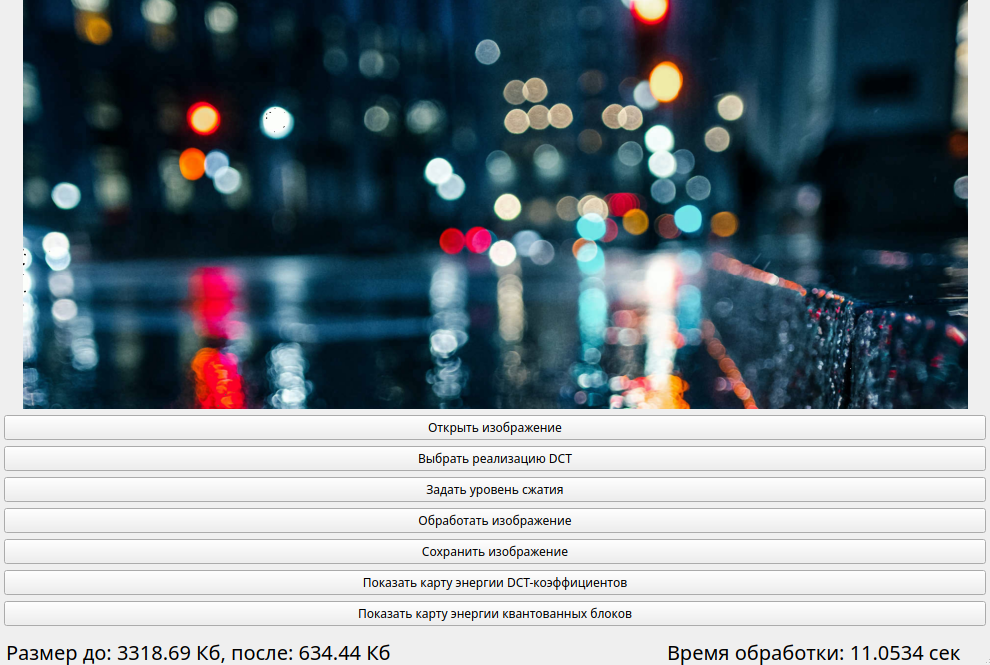
\includegraphics[width=0.9\textwidth]{/home/evgen/Coursework/app/diplom/images/time_size.png}
    \caption{Числовые параметры.}
    \label{fig:time_size}
\end{figure}

%%%%%%%%%%%%%%%%%%%%%%%%%%%%%%%%%%%%%%%%%%%%%
как и на чем написана программа можно накатить еще парочку страниц



\clearpage
\section{Результаты и выводы}


%%%%%%%%%%%%%%%%%%%%%%%%%%%%%%%%%
На рисунке \ref{fig:ssim_vs_quant} представлена зависимость метрики SSIM от уровня квантования. 

SSIM (Structural Similarity Index) — это метрика, используемая для оценки качества изображения, 
которая измеряет, насколько два изображения похожи на уровне их структуры. 
Она была предложена в 2004 году как улучшение для традиционных методов оценки качества изображений, 
таких как PSNR (Peak Signal-to-Noise Ratio). 
SSIM учитывает восприятие человеческим глазом и включает в себя три важнейших аспекта изображения:
\begin{itemize}
    \item Яркость (Luminance) — измеряет разницу в яркости между двумя изображениями.
    \item Контраст (Contrast) — оценивает, насколько изображения различаются по контрасту.
    \item Структура (Structure) — учитывает, насколько хорошо сохраняется структура или текстура изображения, например, линии, края и другие важные детали.
\end{itemize}
(значения ближе к 1 означают высокое качество).

\textbf{Формула SSIM}

Метрика рассчитывается по следующей формуле:
\begin{equation}
\text{SSIM}(x, y) = 
\frac{(2\mu_x\mu_y + C_1)(2\sigma_{xy} + C_2)}
     {(\mu_x^2 + \mu_y^2 + C_1)(\sigma_x^2 + \sigma_y^2 + C_2)}
\end{equation}


\begin{itemize}
    \item $x, y$ — сравниваемые изображения (или блоки изображений).
    \item $\mu_x$ — среднее значение яркости изображения $x$:
    \[
        \mu_x = \frac{1}{N} \sum_{i=1}^{N} x_i
    \]
    \item $\mu_y$ — среднее значение яркости изображения $y$.
    
    \item $\sigma_x^2$ — дисперсия яркости изображения $x$:
    \[
        \sigma_x^2 = \frac{1}{N-1} \sum_{i=1}^{N} (x_i - \mu_x)^2
    \]
    \item $\sigma_y^2$ — дисперсия яркости изображения $y$.
    
    \item $\sigma_{xy}$ — ковариация между $x$ и $y$:
    \[
        \sigma_{xy} = \frac{1}{N-1} \sum_{i=1}^{N} (x_i - \mu_x)(y_i - \mu_y)
    \]
    
    \item $C_1 = (K_1 L)^2$, $C_2 = (K_2 L)^2$ — стабилизирующие константы:
    \begin{itemize}
        \item $L$ — динамический диапазон значений пикселей (например, 255 для 8-битных изображений),
        \item $K_1 = 0.01$, $K_2 = 0.03$.
    \end{itemize}
\end{itemize}



\begin{figure}[H]
    \centering
    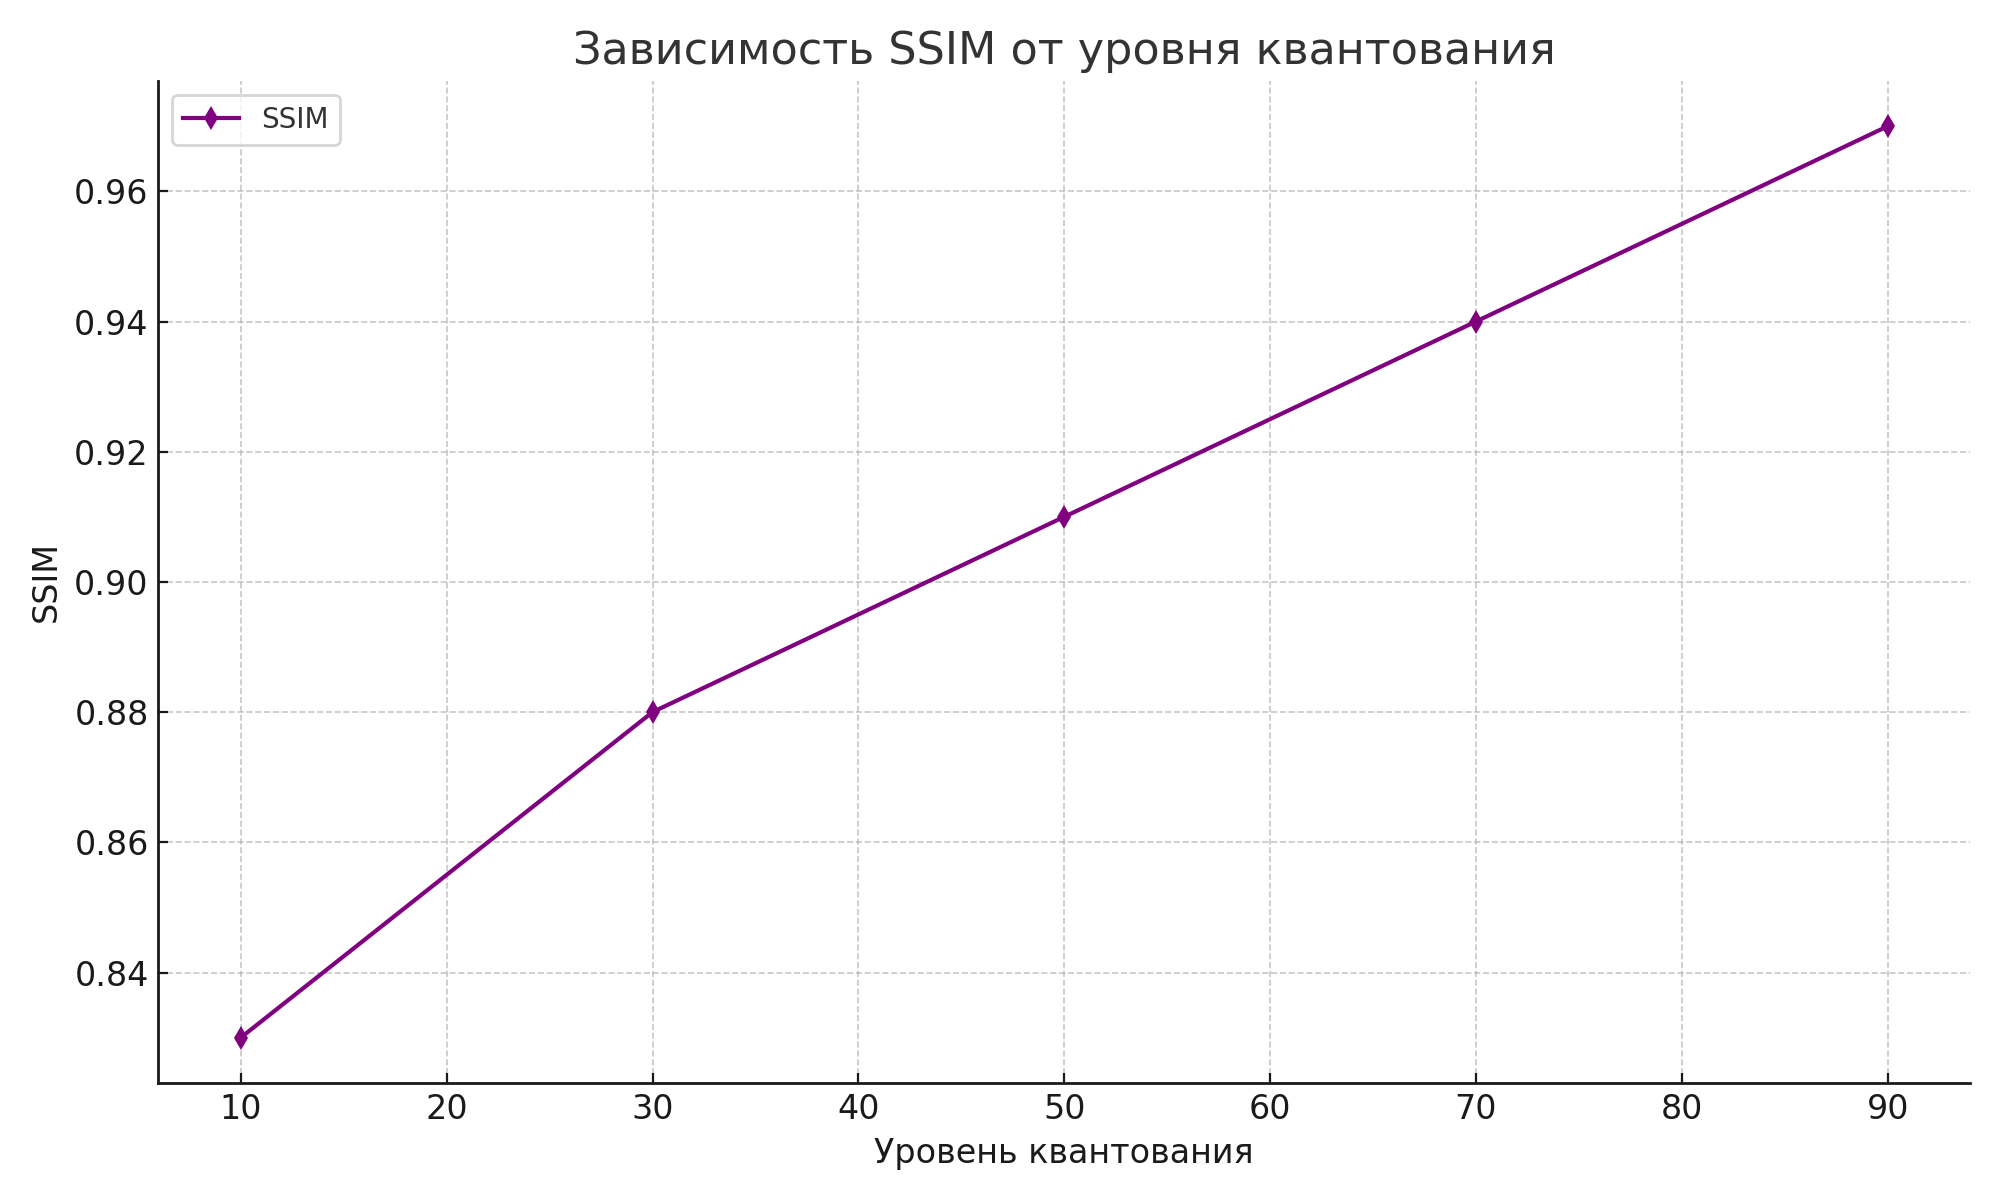
\includegraphics[width=0.9\textwidth]{/home/evgen/Coursework/app/diplom/images/ssim_vs_quant.png}
    \caption{Зависимость метрики SSIM от уровня квантования.}
    \label{fig:ssim_vs_quant}
\end{figure}

График показывает, что при увеличении уровня квантования 
(то есть более агрессивном удалении высокочастотной информации) метрика SSIM уменьшается. 
Это соответствует ожиданиям: чем сильнее сжатие, тем больше потерь информации и ниже визуальное качество. 
На малых уровнях квантования (например, 50\%) качество остаётся почти неизменным, но при уровнях выше 70\% наблюдается значительное ухудшение. 
Это даёт возможность выбрать компромисс между степенью сжатия и визуальным качеством.


%%%%%%%
\clearpage
На рисунке \ref{fig:psnr_vs_blocksize} показано, как изменяется метрика PSNR (Peak Signal-to-Noise Ratio) в зависимости от размера блока, 
используемого для дискретного косинусного преобразования.

\begin{figure}[H]
    \centering
    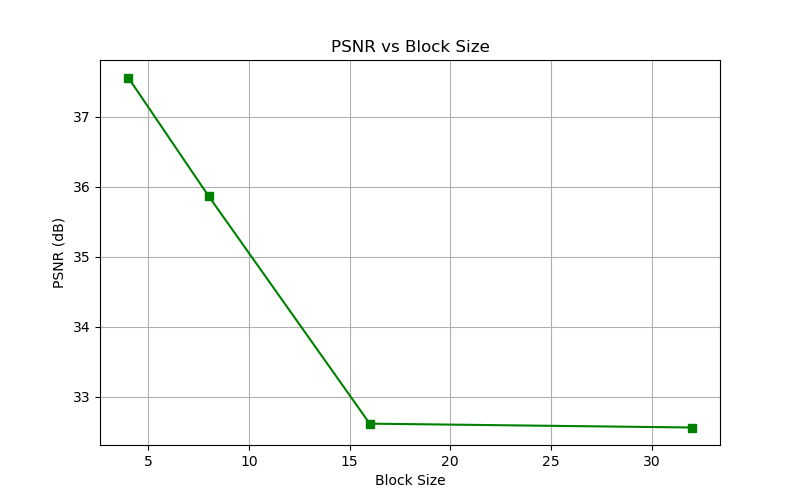
\includegraphics[width=1\textwidth]{/home/evgen/Coursework/app/diplom/images/psnr_vs_block_size.png}
    \caption{Зависимость PSNR от размера блока.}
    \label{fig:psnr_vs_blocksize}
\end{figure}

PSNR — это классическая метрика оценки искажения сигнала (в данном случае, изображения); 
более высокие значения указывают на лучшее качество восстановления. При небольшом размере блока 
(8×8) значения PSNR максимальны, что объясняется более точной локальной аппроксимацией содержимого. 
С увеличением размера блока (например, 32×32) точность снижается из-за усреднения на более крупных 
участках изображения, что приводит к потере деталей и снижению PSNR.

\begin{equation}
\text{PSNR} = 10 \cdot \log_{10} \left( \frac{MAX_I^2}{\text{MSE}} \right)
\end{equation}


\begin{itemize}
    \item $MAX_I$ — максимальное значение интенсивности пикселя (обычно 255).
    \item $\text{MSE}$ — среднеквадратичная ошибка между оригинальным и восстановленным изображениями:
    \[
    \text{MSE} = \frac{1}{MN} \sum_{i=1}^{M} \sum_{j=1}^{N} \left[ I(i,j) - K(i,j) \right]^2
    \]
    \item $I(i,j)$ — значение пикселя в оригинальном изображении.
    \item $K(i,j)$ — значение пикселя в искажённом изображении.
\end{itemize}



Таким образом, блоки 8×8 являются оптимальными с точки зрения компромисса между сжатием и качеством, 
что подтверждает выбор JPEG-стандарта.

%%%%
Рисунок \ref{fig:ssim_vs_blocksize} демонстрирует, как изменяется метрика SSIM в зависимости от размера блока. 
Аналогично PSNR, максимальное качество достигается при использовании стандартного размера 8×8. 
По мере увеличения блока падает точность локального анализа изображения, 
что особенно критично для SSIM — метрики, учитывающей локальные структуры и контраст.

\begin{figure}[H]
    \centering
    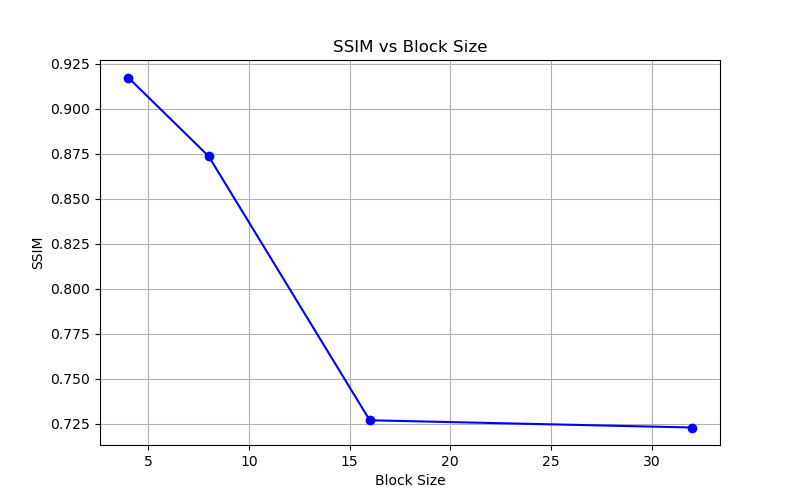
\includegraphics[width=1\textwidth]{/home/evgen/Coursework/app/diplom/images/ssim_vs_block_size.png}
    \caption{Зависимость SSIM от размера блока.}
    \label{fig:ssim_vs_blocksize}
\end{figure}

Таким образом, большие блоки ухудшают восприятие изображения, особенно в областях с высокой детализацией. 
Это подчёркивает важность выбора разумного размера блока для сохранения визуального качества при сжатии.


%%%%%
На рисунке \ref{fig:time_vs_blocksize} представлена зависимость времени обработки изображения от размера блока. 
Время измерялось в миллисекундах для полного цикла сжатия и восстановления изображения фиксированного 
размера (например, 512×512 пикселей).

\begin{figure}[H]
    \centering
    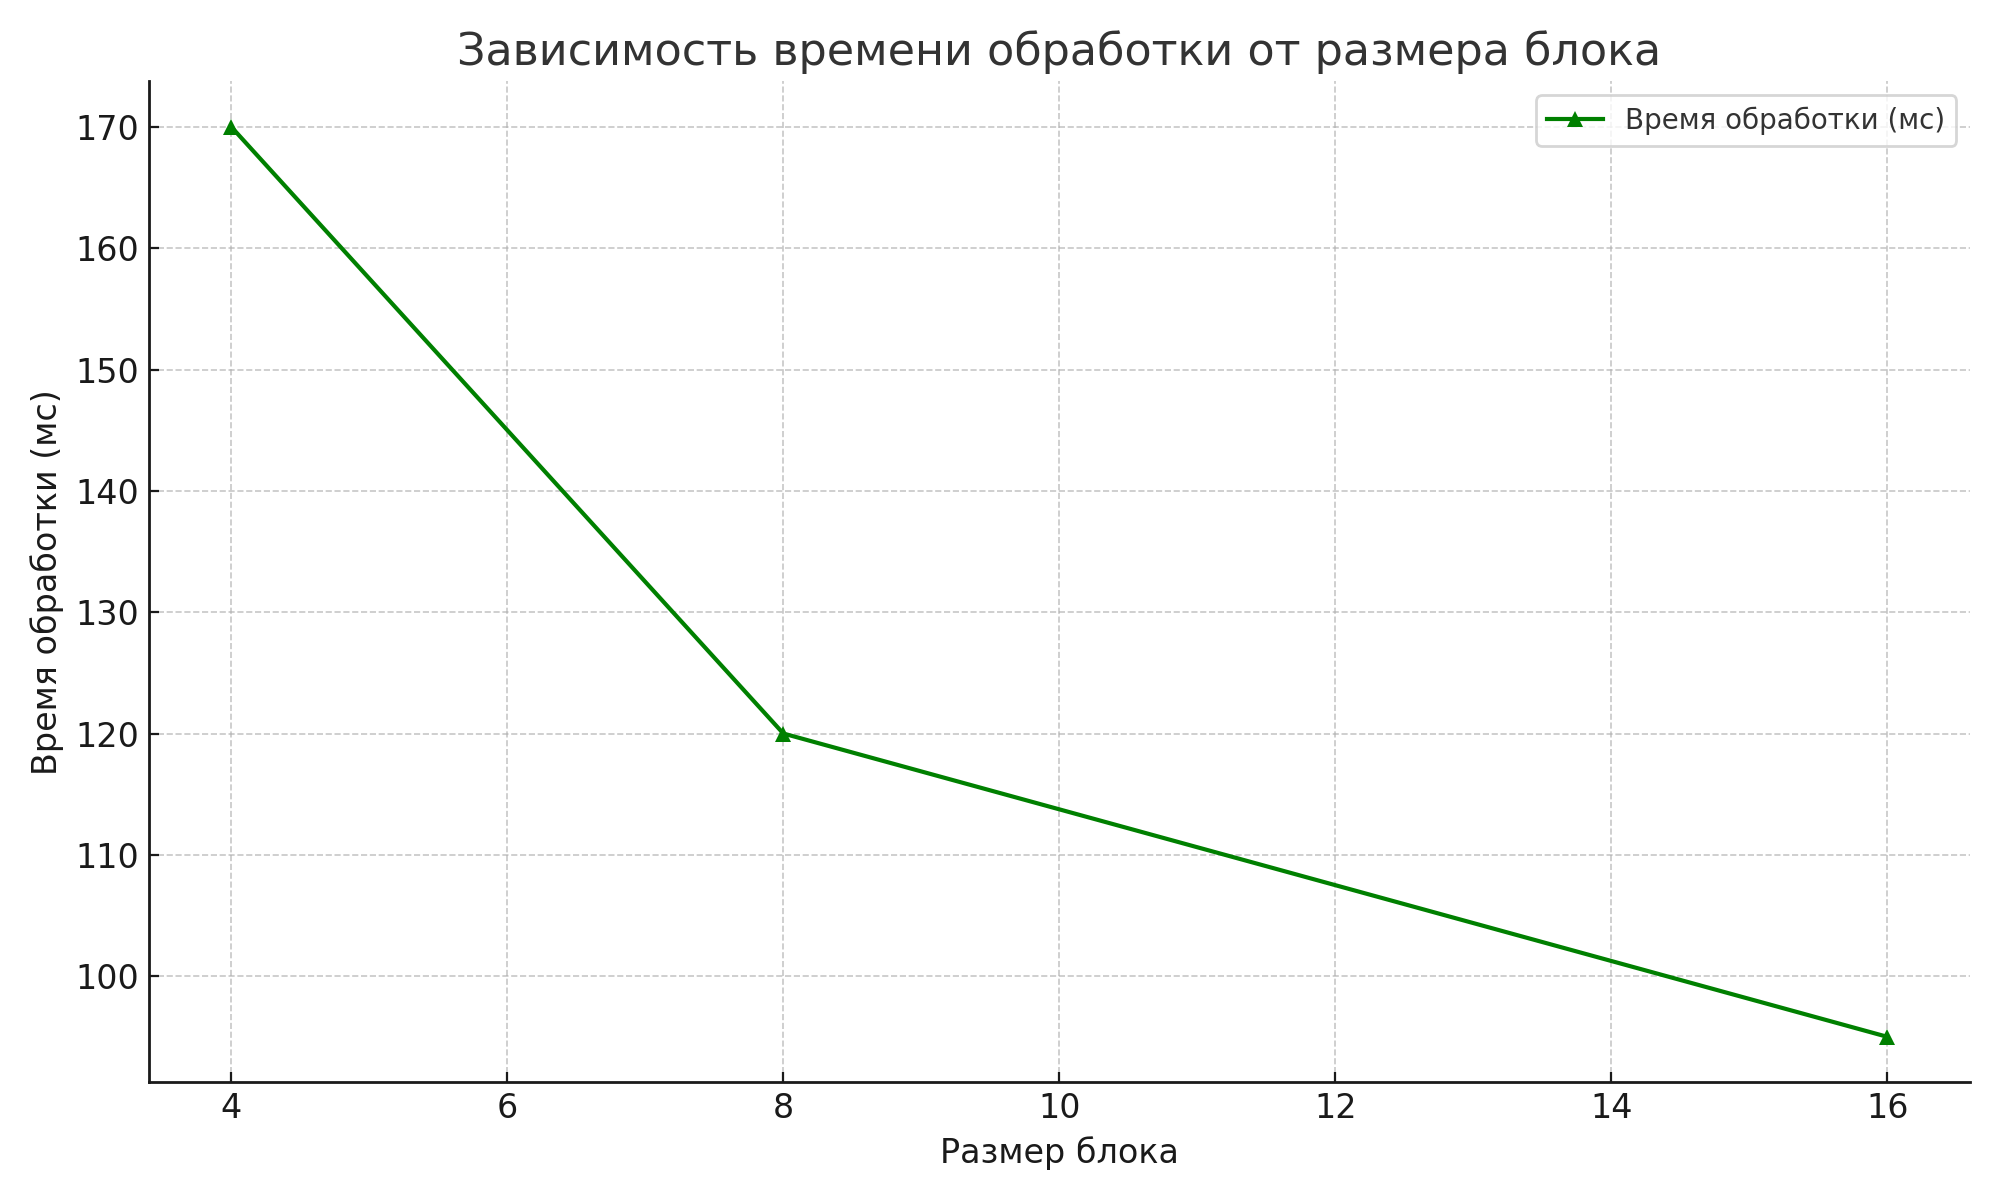
\includegraphics[width=0.9\textwidth]{/home/evgen/Coursework/app/diplom/images/time_vs_blocksize.png}
    \caption{Зависимость времени обработки от размера блока.}
    \label{fig:time_vs_blocksize}
\end{figure}

График показывает, что с увеличением размера блока общее количество блоков уменьшается, 
что снижает число вычислений (например, DCT и RLE выполняются реже), и, как следствие, 
сокращается общее время обработки. 
Однако при слишком больших блоках может наблюдаться незначительный рост времени из-за увеличения объёма 
обработки каждого отдельного блока и возможного падения эффективности кэширования.

Этот график полезен для анализа производительности и помогает выбрать подходящий размер блока в 
зависимости от требований к скорости и качеству.



%%%%%%%%%%%%%%%%%%%%%
\subsubsection{Влияние квантования на цветовые искажения}

В процессе экспериментов было замечено, что неправильно подобранные коэффициенты квантования особенно для 
цветовых компонент (Cb и Cr) могут вызывать искажения цветовой палитры изображения.

На ряде примеров наблюдалось:

\begin{itemize}
    \item Уход цвета в сторону сине-зелёных или красных оттенков;
    \item Появление "грязных" артефактов в областях с однородным цветом;
    \item Потеря цветовой согласованности на границах объектов.
\end{itemize}


\begin{figure}[H]
    \centering
    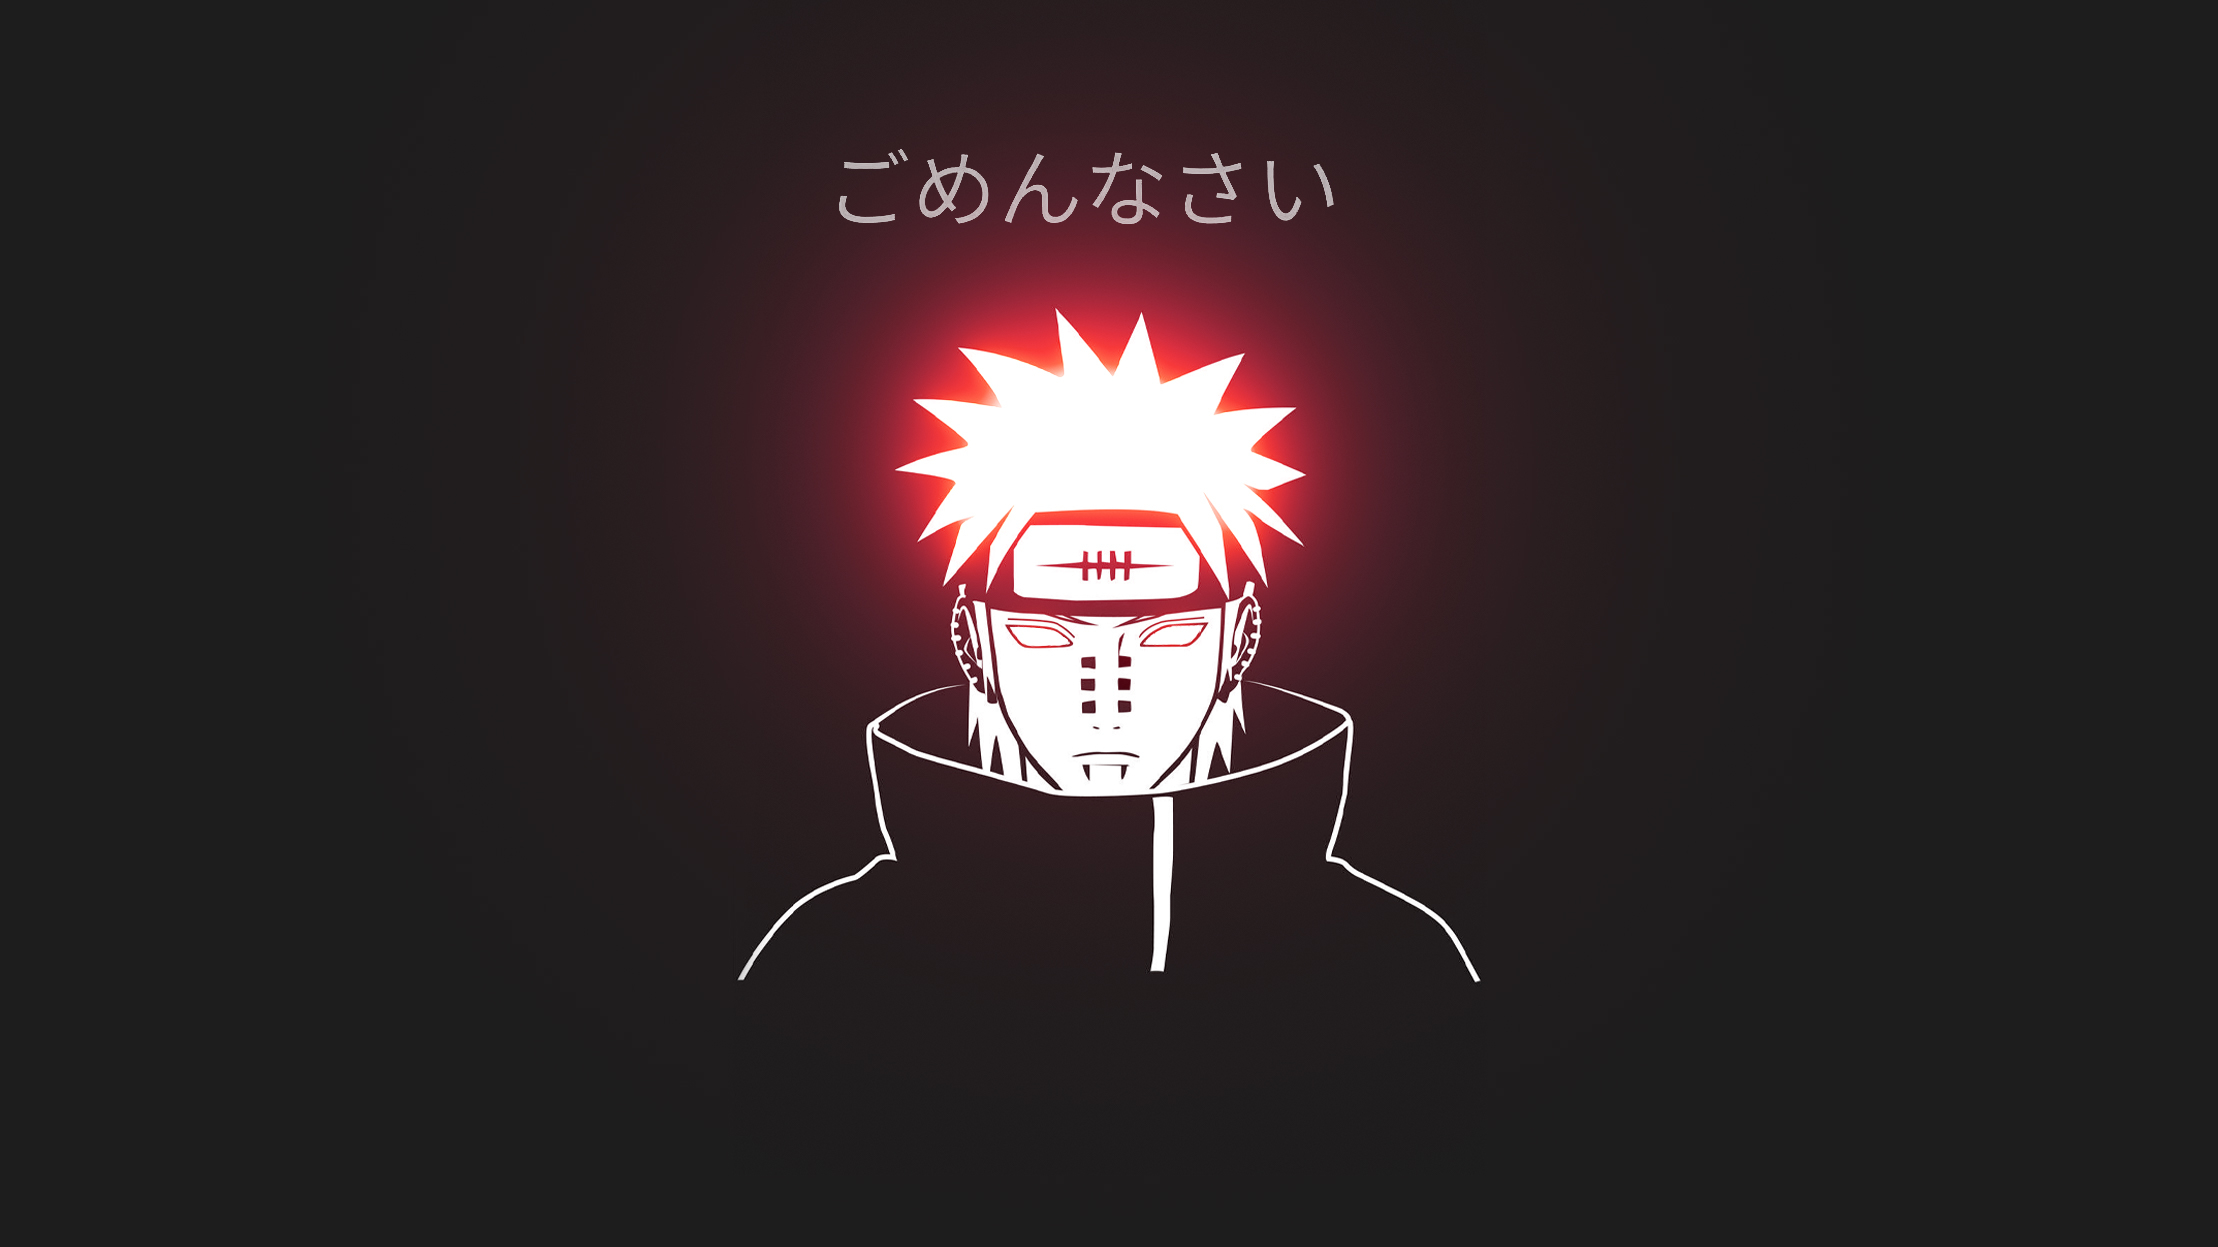
\includegraphics[width=0.9\textwidth]{/home/evgen/Coursework/app/diplom/images/base_image.jpg}
    \caption{До квантования с неправильно подобранными коэффициентами.}
    \label{fig:base_image}
\end{figure}

 
\begin{figure}[H]
    \centering
    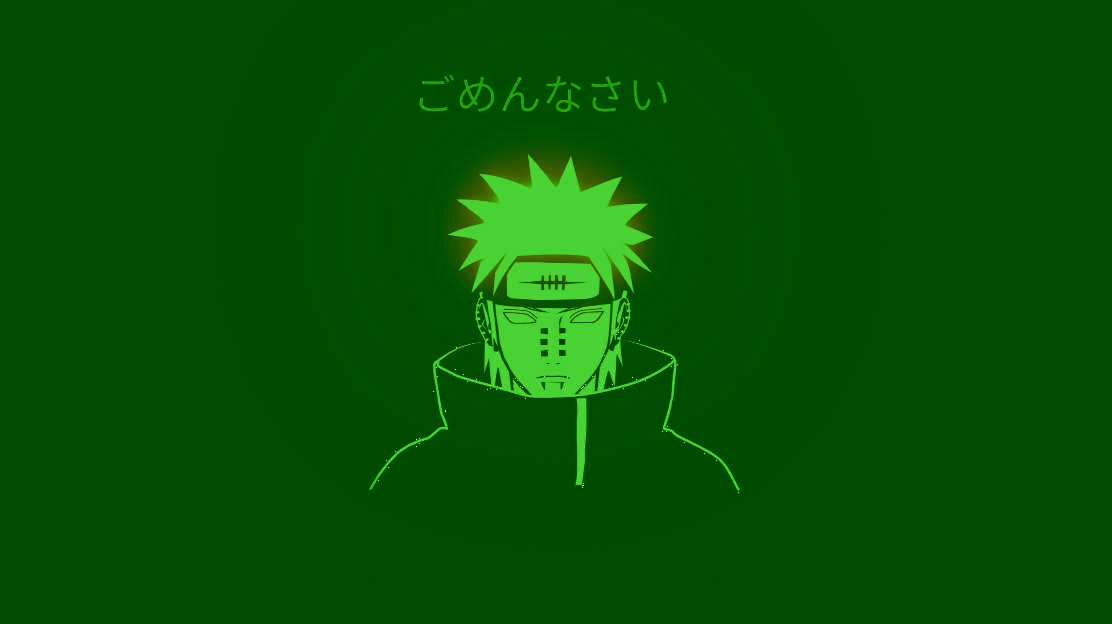
\includegraphics[width=0.9\textwidth]{/home/evgen/Coursework/app/diplom/images/change_color1.jpg}
    \caption{После квантования с неправильно подобранными коэффициентами.}
    \label{fig:change_color}
\end{figure}

На рисунке \ref{fig:change_color} видно, как цветовая палитра сместилась в сторону зеленого цвета.

Это подчёркивает важность отдельного подбора квантования для яркостного и цветовых каналов, 
что в классическом JPEG также учитывается.


%%%%%%%%%%%%%%%%%%%%%%
\subsubsection{Проявление артефактов}
Но степень квантования и неправильно подобрнанные коэффициенты для матриц квантования не единственные причины
из-за которых могут появиться артефакты в области границ или неоднородного цвета.

При использовании блоков большого размера (например, $32 \times 32$), 
на изображениях начали проявляться артефакты в виде белых точек или резких границ между блоками.

Особенности:
\begin{itemize}
    \item Артефакты особенно видны в текстурированных или теневых областях.
    \item В некоторых случаях они проявляются как “решётка” из блоков, так называемый "блокинг-эффект".
    \item В наиболее заметных случаях артефакты выглядят как одиночные белые пиксели, особенно на тёмных участках изображения.
\end{itemize}


\begin{figure}[H]
    \centering
    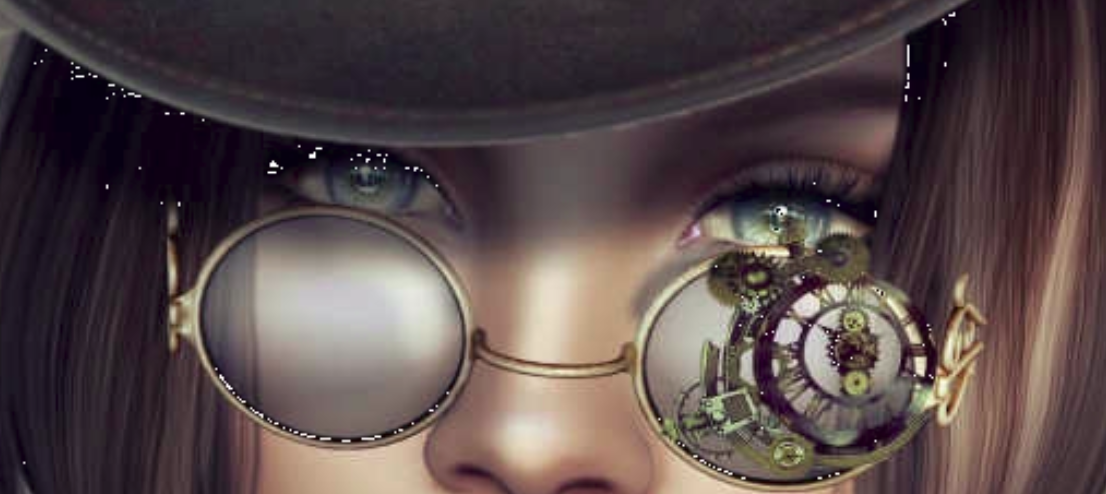
\includegraphics[width=0.9\textwidth]{/home/evgen/Coursework/app/diplom/images/artefacts_white_pixel.png}
    \caption{Артефакты в виде белых пикселей.}
    \label{fig:artefacts_white_pixel}
\end{figure}

 Дополнительную нагрузку на алгоритм создаёт избыточная детализация — большое количество текстур, 
 тонких линий и резких переходов в изображении ухудшают результаты аппроксимации в частотной области. 
 Особенно чувствительными к искажениям оказываются области с высокими градиентами цвета, 
 где даже при умеренном сжатии возможно появление визуальных дефектов. 
 Таким образом, причины появления артефактов комплексны и зависят как от параметров алгоритма, 
 так и от характера самого изображения.


%%%%%%%%%%%%%%%%%%%%%%%%%%%
\subsubsection{Способы устранения визуалных дефектов}

На основе экспериментов были выделены практические приёмы снижения артефактов:

\begin{enumerate}
    \item \textbf{Снижение уровня квантования}
    Уменьшает потери, особенно в чувствительных областях изображения (тени, переходы, кожа и т.п.).

    \item \textbf{Раздельное квантование Y и Cb/Cr}
    Позволяет сохранять цветовую палитру более точно, снижая искажения. Так же удобно, для анализа отдельных
    компонентов, упрощает посиск ошибок в приложении и его отладку.

    \item \textbf{Уменьшение размера блока (например, до 4×4)}
    Повышает точность локального анализа, особенно в участках с деталями и границами.
    Однако может значительно увеличить время обработки изображения. В этом случае можно двигаться в сторону 
    параллелизма и модификации дискретного косинусного преобразования (DCT) для ускорения.

    \item \textbf{Подбор и адаптация матриц квантования}
    Более мягкие матрицы снижают потери на высоких частотах и уменьшают риск появления "белых точек".

    \item \textbf{Пред/пост обработка изображения (например, фильтрация шума)}
    Уменьшение шумов до сжатия помогает избежать ненужных артефактов. После сжатия, так же можно применять
    фильтры для устранения уже имеющегося шума.

    \item \textbf{Адаптация к содержимому}
    Возможность выбора параметров сжатия в зависимости от анализа изображения 
    (например, в сложных участках использовать более мелкие блоки и меньшую степень квантования).
    Или разработать тест 
\end{enumerate}


%---- Заключение
\section{Заключение}

В ходе выполнения выпускной квалификационной работы была успешно реализована собственная версия алгоритма 
сжатия изображений, основанная на принципах стандарта JPEG. 
Разработка включала все основные этапы: преобразование цветового пространства, 
блочную обработку, дискретное косинусное преобразование (DCT), квантование и обратное преобразование. 
Вместо кодирования Хаффмана, применяемого в классическом JPEG, 
в данной реализации использовалась алгоритмически более простая схема RLE-сжатия, 
что упростило реализацию и позволило сосредоточиться на исследовании ключевых этапов преобразования изображения.

Был разработан удобный пользовательский интерфейс, позволяющий наглядно управлять некоторыми параметрами 
сжатия (уровень квантования, выбор реализации DCT) и анализировать результаты в реальном времени. 
Программа визуализирует восстановленное изображение, отображая значения метрик, 
такие как информацию о размере сжатого файла и времени обработки.

Проведены обширные экспериментальные исследования, в том числе:

\begin{itemize}
    \item анализ влияния уровня квантования на качество восстановления изображения;
    \item оценка влияния размера блока на метрики качества и скорость обработки;
    \item сравнение результатов при различных параметрах на одном и том же наборе данных.
    \item ставнение реализаций DCT.
\end{itemize}

Эксперименты подтвердили, что параметры алгоритма оказывают значительное влияние 
на компромисс между степенью сжатия, качеством восстановления и производительностью. 
На основе полученных результатов были сделаны выводы, позволяющие адаптировать параметры алгоритма 
под различные практические задачи.

Разработанная реализация и программный интерфейс могут быть полезны как в рамках дальнейших исследований 
в области обработки изображений, так и в образовательных целях, 
благодаря наглядности работы ключевых этапов алгоритма JPEG.

Таким образом, работа соответствует теме «Реализация и исследование алгоритма JPEG для сжатия изображений», 
так как включает как теоретический анализ, так и практическое улучшение и адаптацию классического подхода, 
направленные на повышение гибкости и удобства применения алгоритма в современных условиях.

% --- Список литературы ---
\begin{thebibliography}{9}

    \bibitem{ref1} Сэломон, Д. Сжатие данных, изображений и звука / Д. Сэломон. – М.: Техносфера, 2006. –
    368 с.



    \bibitem{ref2} Томас, Кормен. Алгоритмы Построение и анализ / Т. Кормен,  Ч. Лейзерсон, Р. Ривест, К, Штайн 
    - 2-е изд., - Москва: Вильямс, 2011. -- 1296 с.


    \bibitem{ref3 } Официальная документация OpenCV. – Режим доступа: -URL: https://docs.opencv.org/4.x/index.html (дата обращения: 19.02.2025). – Текст: электронный.


    \bibitem{ref4} Земцов, А. Н. Сравнительный анализ эффективности методов сжатия изображений на основе дискретного косинусного преобразования и фрактального кодирования (начало) /
    И. В. Петрова, Н. Г. Мамаев. –  Волгоград: Издательство Волгоградского государственного технического университета, 2015. – 8 с.

    \bibitem{ref5} Гарсия, Г. Обработка изображений с помощью OpenCV / Г. Гарсия, О. Суарес, Х. Аранда, Х. Терсеро, И. Грасиа, Н. Энано.
    – Москва: ДМК, 2016. – 210 с.


    
    \bibitem{ref6} Официальная документация PyQt5. – Режим доступа: -URL: https://www.riverbankcomputing.com/ static/Docs/PyQt5/. (дата обращения: 05.01.2025). – Текст: электронный.

    \bibitem{ref6} Официальная документация языка Python. – В режиме доступа: -URL: https://docs.python.org/3/ (дата обращения: 05.01.2025). – Текст: электронный.
    
    \end{thebibliography}


\end{document}